\documentclass[10pt,letterpaper]{book}

\usepackage{outlines}
\usepackage{amsmath}
\usepackage{tikz}
\usepackage{hyperref}
\usepackage{enumitem}

\usepackage{subcaption}
\DeclareCaptionOptionNoValue{centering}{\centering} % Make sure everything is centered in subs
\captionsetup[sub]{centering}

\usepackage{multirow}
\usepackage{cancel}
\usepackage{float}

\usepackage{parskip}

\usepackage{slantsc,lmodern}

\usepackage{pgfplotstable,booktabs}
\usepackage{framed}
\definecolor{shadecolor}{rgb}{0.9,0.9,0.9}

\usepackage{gensymb}

\usepackage{paralist}

\usepackage[paper=a4paper,margin=1in]{geometry}

\usepackage{etoolbox}

%\addtolength{\oddsidemargin}{-.875in}
%\addtolength{\evensidemargin}{-.875in}
%\addtolength{\textwidth}{1.75in}

%\addtolength{\topmargin}{-.875in}
%\addtolength{\textheight}{1.75in}

% Centers all the floats
\makeatletter
\g@addto@macro\@floatboxreset\centering
\makeatother

\begin{document}


\clearpage
%% temporary titles
% command to provide stretchy vertical space in proportion
\newcommand\nbvspace[1][3]{\vspace*{\stretch{#1}}}
% allow some slack to avoid under/overfull boxes
\newcommand\nbstretchyspace{\spaceskip0.5em plus 0.25em minus 0.25em}
% To improve spacing on titlepages
\newcommand{\nbtitlestretch}{\spaceskip0.6em}
\pagestyle{empty}
\begin{center}
  \bfseries
  \nbvspace[1]
  \Huge
  {\nbtitlestretch\huge
    MECHATRONICS}

  \nbvspace[1]
  \normalsize
  TECHNOLOGIES, PRINCIPLES, DESIGN, AND ANALYSIS\\
  OF COMPLEX ELECTRO-MECHANICAL SYSTEMS\\
  
  \nbvspace[1]
  \small BY\\
  \Large THADDEUS HUGHES\\[0.5em]

  \nbvspace[2]

  \nbvspace[3]
  \normalsize

  \large
  PUBLISHED IN THE WILD \\
  \small APRIL 2020 \\
\end{center}

\newgeometry{top=0.75in,bottom=0.75in,right=0.75in,left=1.25in}

\raggedbottom

\tableofcontents

\chapter{Introduction}
 
 {\slshape \scshape ``You have to be in a state of play to design. If you're not in a state of play, you can't build anything." - Paula Scher}

Mechatronics is an amalgam of mechanical electronics - systems that contain both mechanical and electrical components. It's a field that spans nearly every industry, so any one source (even this one) will not be complete with all the information you need. But this may be a good jumping off point. I'm writing this generally towards those in a competitive robotics environment, so will use many examples from there, but you soon find that those same technologies that shoot foam balls into goals can be used anywhere from assembly lines to emergency medical equipment.

This document is not intended to be all-encompassing. It is no bible. In reality, it's just an outline; a map if you will. We live in an era where information is readily available on net demand. This document really doesn't contain anything new. Its goal is to show you a plethora of things that exist in a breadth-first fashion before you dive down a particular rabbit hole. There are a few places where I'll dive deeper because I feel it's relevant to show you some of the nuances you should be aware of. By and large, my goal isn't to drill home every single thing- because I'll fail at that. Someone will come up with something new, or improve something discussed here, and this information will become outdated. I'll try to keep it up to date... but I will definitely fail!

The human mind is a weird thing. It's better at prompted recall than unprompted recall. You may not always be thinking about the many different types of bolts, but if you've seen that before, and you come across a problem that needs that information, you'll find you might be able to figure it out- or at least know where to start looking.

I hope to keep this terse. We're going to go fast and I'm going to leave some things to your imagination or research to figure out exactly how they work. Mechatronics is what I love, so I don't want to spoil it by chewing your steak for you. With that... let's begin.

\chapter{Construction}
 
 {\slshape \scshape ``The first little pig was very lazy. He didn't want to work at all and he built his house out of straw. The second little pig worked a little bit harder but he was somewhat lazy too and he built his house out of sticks. The third little pig worked hard all day and built his house with bricks. It looked like it could withstand the strongest winds." - English Folk Tale}
 
 The parable of the three little pigs reminds us that how we build things is important. And while at first blush, the story seems to be about how you should always build strong out of brick, sometimes we should learn from the first pig, and build fast for prototyping. Having a suite of different fabrication techniques at hand can be incredibly handy.
 
 \section{Materials}
 
 Everything is made from materials. There are a lot of different materials out there, all with different properties. Some are natural, some are completely synthetic, but all can be measured, quantified, and compared. Important properties we'll focus on are:
 
 \begin{compactitem}
 	\item Density (weight)
 	\item Stiffness
 	\item Hardness
 	\item Strength
 	\item Toughness
 	\item Thermal capabilities
 	\item Frictional and chemical interactions
 \end{compactitem}
 
 You'll notice that stiffness, strength, hardness, and toughness are all different characteristics. They are distinctly different properties in engineering.
 
 To show this, we'll first consider a \textit{stress-strain curve}. This curve is created by pulling on a specimen of material like shown, interpreting the force and deflection data into \textit{stress} $\sigma$ (force per cross-sectional area) and \textit{strain} $\epsilon$ (percent deflection).
 
 \begin{figure}[H] \centering
 	\begin{tikzpicture}[x=1.0in, y=1.0in]
 		\draw[ ] (-0.1,0) -- (0.1,0) -- (0.1, 1) -- (-0.1, 1) -- cycle;
 		\draw[->] (0,-0.1)--(0,-0.5) node[pos=0.5, right]{$F$};
 		\draw[->] (0,1.1)--(0,1.5) node[pos=0.5, right]{$F$};
 	\end{tikzpicture}
 	\qquad
 	\begin{tikzpicture}[x=1.0in, y=1.0in]
 		\draw[->] (0,0)--(3,0) node[pos=0.5, below]{$\epsilon$};
 		\draw[->] (0,0)--(0,2) node[pos=0.5, left]{$\sigma$};
 		\draw[blue, thick] (0,0)--(1,1);
  		\draw[gray] (1,1)--(1.8,1.8);
 		\draw[red, thick]  (1,1) .. controls (1.5,1.5) and (2.0,1.5) .. (2.5,1.25);
 		\draw[purple, ->] (2,1.4)--(0.6,0);
 	\end{tikzpicture}
 \end{figure}
 
 The portion of the curve that is linear (highlighted in blue) is referred to as the 'elastic' portion. When the material is operating in this region, it will always snap back (think of a spring). If, however, we dip into the red portion of the curve (called the 'plastic' portion), when we release the material, it will have permanently deformed (following the purple arrow).
 
 The key aspects of the curve can be boiled down into a few properties.
 
 \begin{asparaenum}[a)]
 	\item \textit{Young's Modulus}, or the \textit{Elastic Modulus} ($E$) is the slope of the elastic portion of the curve. A higher $E$ denotes a stiffer material.
 	\item \textit{Yield strength} ($\sigma_{y}$) is the highest stress seen in the elastic portion of the curve.
 	\item \textit{Ultimate tensile strength} ($\sigma_{UTS}$) is the highest stress the material can see.
 	\item \textit{Percent elongation at break} is the highest strain seen by the material before it breaks. A higher elongation means the material is more 'ductile', while a smaller one means the material is more 'brittle'.
 	\item \textit{Modulus of toughness} is a measure of how much energy the material can absorb. It can be visualized as the area under the curve (think about a shock absorber- it deforms a lot while resisting the load, so can absorb a lot of energy). Materials that are brittle have low toughness.
 \end{asparaenum}
 

 \textit{Hardness} is a property of a material's surface- how much it will permanently indent or scratch. It is not measured by this graph (although it does have some correlations), and is a relative, rather than absolute measurement. There are many different scales. You may have heard of the Mohs scale, introduced to determine the hardness of different minerals based on which can scratch each other. However, most engineering measures will work by indenting an object and measuring how much of an indentation was left behind, which allows for a higher degree of quantization. There are many different scales that are better suited to different materials.
 
 Brinell and Rockwell scales are well suited to metals.
 
 \begin{figure}[H]
 	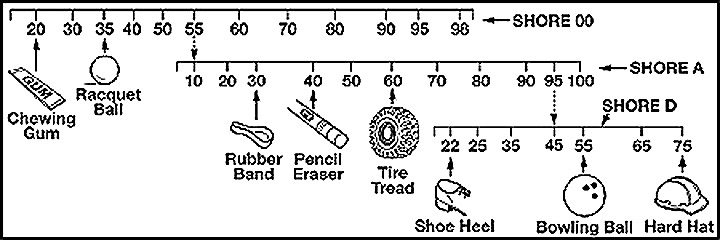
\includegraphics[width=0.85\textwidth]{imgs/shore_hardness.jpeg}
 	\caption{Shore Hardness scales, with some examples}
 \end{figure}
 
 \textit{Shore} AKA \textit{Durometer} scales are suited to measuring elastomers (i.e. rubber). Again it is important to note there are different scales. 90A is much softer than 90D durometer, although they look like they are the same on the above chart, material rated as 95A may be quite different than 45D.
 
 Elastomers are much harder to measure in other ways, and are often given ratings only by their durometer. While this is technically only a measure of hardness, it correlates reasonably well to other material properties like overall stiffness (harder being stiffer) and grip (softer being more interactive, or frictional).
 
 The thermal properties of a material are important. There are three main ones to keep in mind if you are dealing with heat:
 \begin{asparaitem}
 	\item \textit{Thermal conductivity} is how well the material transfers heat. If you're designing a heat sink, you want a high thermal conductivity.
 	\item The \textit{melting point} or \textit{glass transition temperature} are temperatures at which the material undergoes fundamental phase changes. You obviously need to make sure your part doesn't outright melt, but you should also have a bit of margin, as the phenomenon called \textit{creep} can cause parts that are at elevated temperatures to deform over time, even though below melting point.
 	\item The \textit{cefficient of thermal expansion} measures how much material expands as it heats up. If you're working with tight-tolerance equipment (or extreme temperatures), you may need to keep an eye on this.
 \end{asparaitem}
  
 Frictional characteristics and chemical interactions are very complex, and if you care about these, will require some research beyond mere datasheets.
 
 To actually get data to make material comparisons,
 \begin{asparaitem}
 	\item \href{http://www.matweb.com/search/DataSheet.aspx?MatGUID=3a2e111b27ef4e5d813bad6044b3f318&ckck=1}{\color{red}\underline{MatWeb}} has a wide range of material properties.
 	\item \href{https://www.makeitfrom.com/}{\color{red}\underline{MakeItFrom}} has a similarly wide range of materials, and includes a comparison tool to help evaluate different options.
 \end{asparaitem}
 
 % IMPROVEMENT: General trends / table
 % IMPROVEMENT: Talk about tempering & hardening, maybe?
 
 \section{Form Factors}
 
 Just because the material you want exists, doesn't mean it's widely available in the shape you want. There are a lot of different shapes that a material may be available in, and there are tradeoffs with each different form factor.
 
 \subsection{Cast from Ingnot}
 
\begin{figure}[H]
	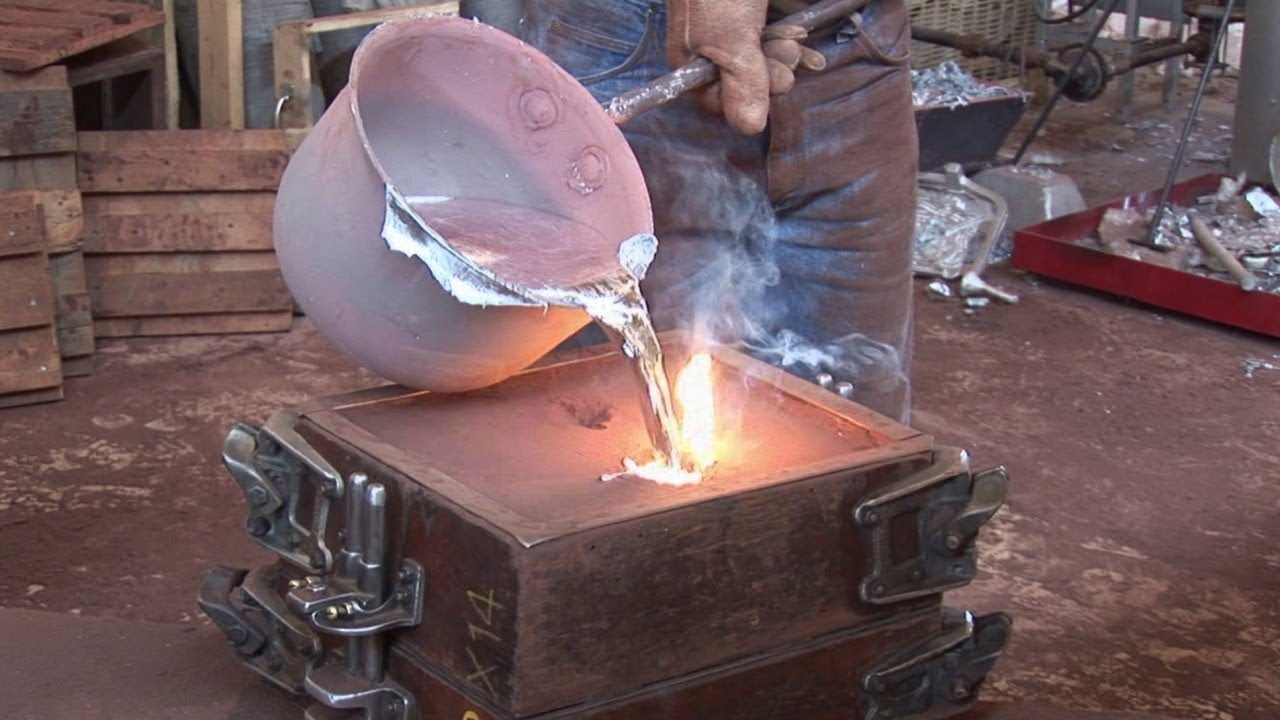
\includegraphics[width=0.55\textwidth]{imgs/casting_proc.jpeg}
	\qquad
	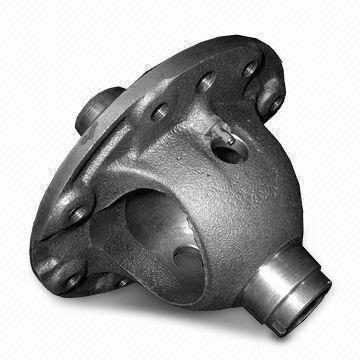
\includegraphics[width=0.3\textwidth]{imgs/casting_part.jpeg}
	\caption{Left: the casting process. Right: A cast differential housing.}
\end{figure} 
 \textit{Casting} is the process of pouring molten material into a mold to produce a complex shape. This shape isn't perfect, as the mold is usually made of sand (in order to withstand the molten metal) and the pouring process can introduce voids and imperfections, so the material properties are usually not as good. Cast parts have notably inferior material properties from billet or forged counterparts.
 
 \subsection{Billet and Plate}
 
 \begin{figure}[H]
	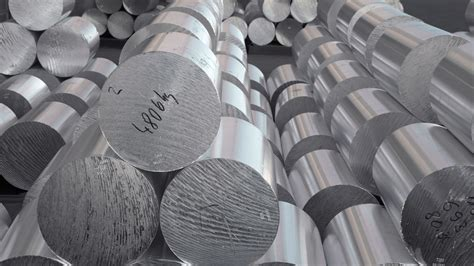
\includegraphics[width=0.6\textwidth]{imgs/billet.jpeg}
	\caption{Pieces of round billet.}
\end{figure} 
 \textit{Billet} material has been poured in a more tightly controlled environment. The resulting material is free of voids and has superior mechanical properties. You can obtain billet plate, bars, or round stock of nearly any material. This material can be held to reasonable tolerances (and by its simple-shaped nature, can be brought into exact dimension by machining quite easily).
 
 \subsection{Extrusions}
 \textit{Extruded} material has been squeezed through a die while molten, and then cooled. Think of a pasta machine. This die can be anywhere from a simple shape like a flat bar, to box tubing, to a very complicated profile with t-slots such as 80/20. Aluminum is the most common material to be extruded. Extrusions have good material properties, and can be held to tight tolerances.
 
  \begin{figure}[H]
	\begin{subfigure}[b]{.24\linewidth}
		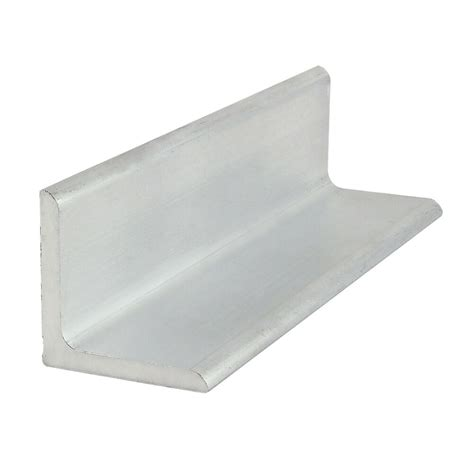
\includegraphics[width=0.95\textwidth]{imgs/extrusion_angle.jpeg}
		\caption{Angles}
	\end{subfigure} \begin{subfigure}[b]{.24\linewidth}
		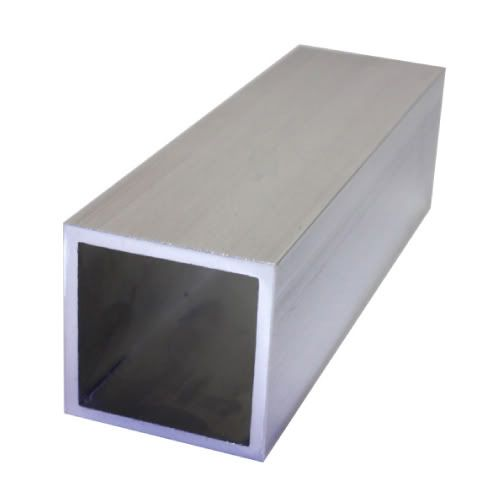
\includegraphics[width=0.95\textwidth]{imgs/extrusion_boxtube.jpeg}
		\caption{Box tube}
	\end{subfigure} \begin{subfigure}[b]{.24\linewidth}
		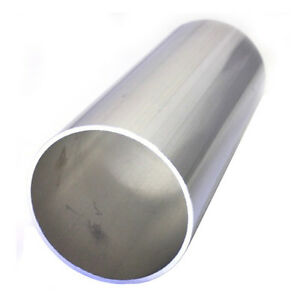
\includegraphics[width=0.95\textwidth]{imgs/extrusion_roundtube.jpeg}
		\caption{Pipe and tube}
	\end{subfigure}	\begin{subfigure}[b]{.24\linewidth}
		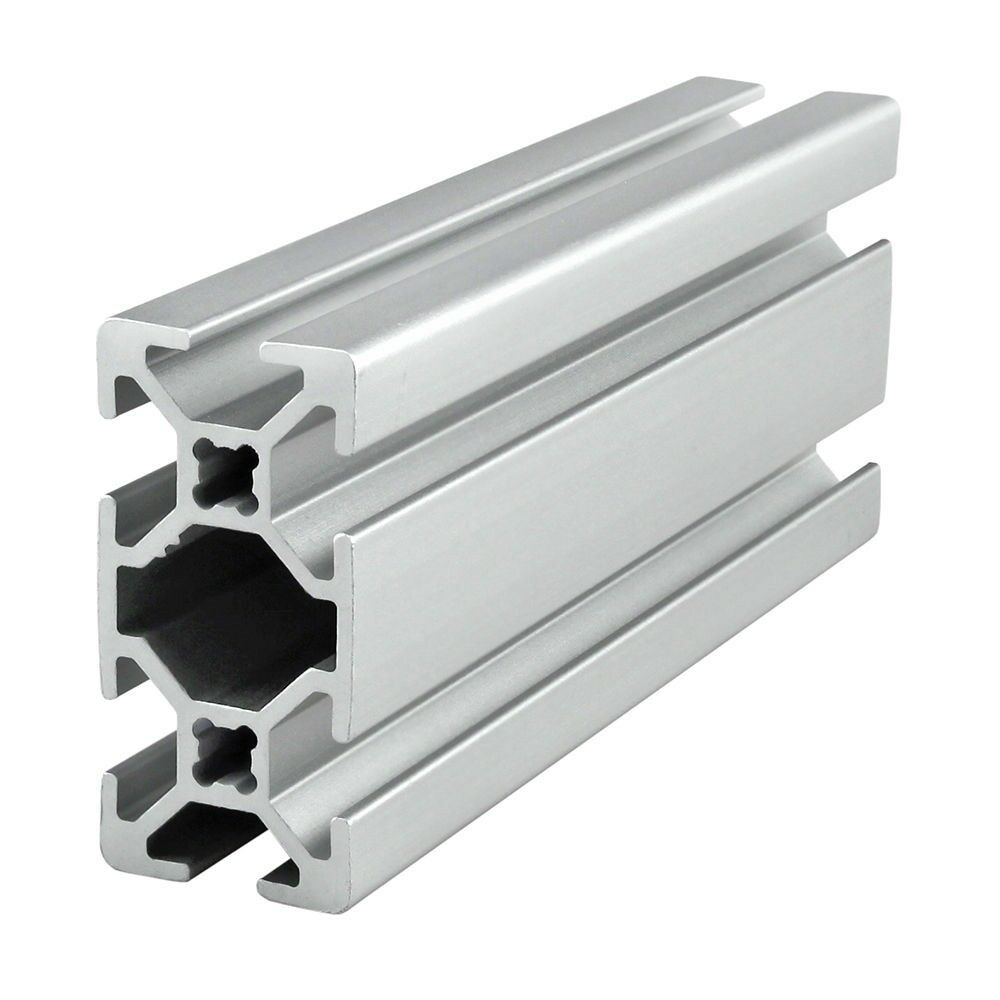
\includegraphics[width=0.95\textwidth]{imgs/extrusion_8020.jpeg}
		\caption{T-slot framing}
	\end{subfigure}	
	\caption{Various Extrusions}
\end{figure}

 \begin{asparaenum}[a)]
 	\item \textit{Angles} are measured by the leg width and the thickness. Only one dimension for leg lengths may be given if the leg lengths are equal. There may or may not be a radius in the corner, and radiuses on the tips of the legs.
 	\item \textit{Box tube} is measured by the outer side lengths and the thickness. It may or may not have an inner or outer radius- if it isn't specified, it probably doesn't.
 	\item \textit{Pipe and tube} is measured either by diameter and thickness, or by nominal pipe size and schedule. `1 inch' tube might refer to 1" nominal pipe, which actually has an inner diameter of 1.049", or a piece of tube with a 1" outer diameter. Make sure you know which you're buying.
 	\item \textit{T-slot framing}, known often by the brand name \textit{80/20}, has several slots on the outside which t-slot nuts can be slid into. This makes creating configurable/adjustable frames easy, although the framing is quite heavy. 
 \end{asparaenum}
 
 \subsection{Welded / DOM tubing}
 Steel is not easily extruded, so to make hollow shapes, must be tackled differently. Steel tubes are usually formed by taking sheet and rolling it into a tube, and then welding it together. This process leaves a weld seam which can produce odd material properties, produce dimensional issues (as when making telescoping tubes), or make manufacturing annoying (as the weld is difficult to drill through). 
 
   \begin{figure}[H]
	\centering
	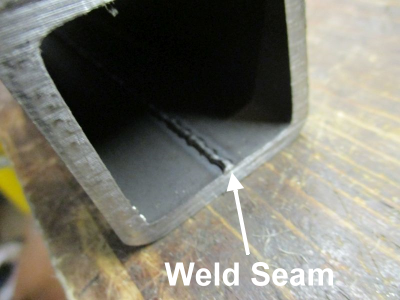
\includegraphics[width=0.4\textwidth]{imgs/welded_tube_seam.png}
	
	\caption{Weld Seam on Tubing}
\end{figure}
 
 \textit{DOM (Drawn-Over-Mandrel)} or \textit{seamless} tubing further processes this tubing to remove the inner seam and produce a product as if it were extruded. It is typically used in demanding applications such as aerospace or motorsport, as well as in components which cannot have a weld seam (such as a reciever hitch, or telescoping tubes).
 
 \subsection{Sheet}
 Material that is sold as 'sheet' rather than 'plate' usually has little-to-no straightness tolerance (in especially thin gagues, it might even be sold as rolls).
 
 \section{Manufacturing Processes}
 
 Once you have a material you like in a shape you can use, you (probably) have to cut or form it into the final shape you want. There are nearly infinite ways of doing this, but here are the most common.
 
 \subsection{Casting/Sintering/Forging}
 
 Casting, sintering, and forging are manufacturing methods which generally require a lot of tooling in order to accomplish, so are generally not suitable for quick-turnaround prototypes such as we need. Some notes, though:
 
 \begin{asparaitem}
 	\item \textit{Casting} as mentioned before, is pouring molten metal into a mold. It can produce very complex shapes (like engine blocks), but the material may end up with lots of voids.
 	\item \textit{Forging} is heating up a metal so that it can be more easily formed, though not liquid. It is then pressed between large dies to form it into the desired shape- essentially, industrialized blacksmithing. Forging can produce fairly complex shapes (like crankshafts), while preserving (and even enhancing) material properties.
 	\item \textit{Sintering} is compressing and heating powder in a mold. Also known as \textit{powder metallurgy}. This can produce somewhat simple parts with good material properties and no draft- many small gears are made this way.
 \end{asparaitem}
 
 \subsection{Machining}
 
 Machining is a broad category of processes that cut material away with a sharp tool. There are many tools that can be used to accomplish this, but there are three that are the most essential and common:
 
 \begin{figure}[H]
	\centering
	\begin{subfigure}[b]{.24\linewidth}
		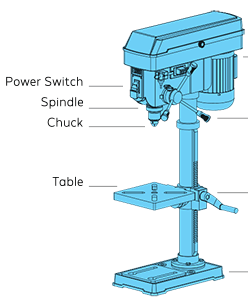
\includegraphics[width=0.95\textwidth]{imgs/drillpress.png}
		\caption{Drill press}
	\end{subfigure}	\begin{subfigure}[b]{.34\linewidth}
		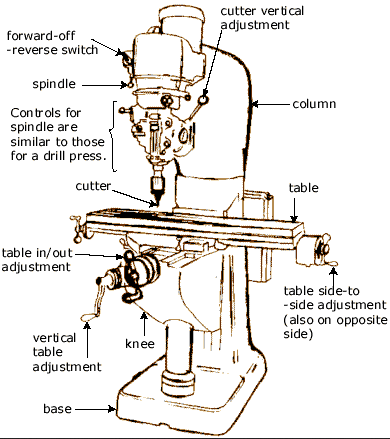
\includegraphics[width=0.95\textwidth]{imgs/mill.png}
		\caption{Milling machine}
	\end{subfigure}	\begin{subfigure}[b]{.4\linewidth}
		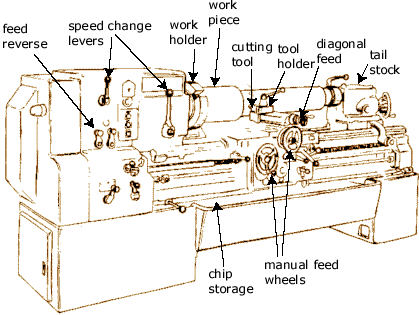
\includegraphics[width=0.95\textwidth]{imgs/lathe.png}
		\caption{Lathe}
	\end{subfigure}	
	
	\caption{The Most Common Machining Tools}
\end{figure}

 \begin{asparaenum}[a)]
 	\item A \textit{drill press} has a rotating spindle and chuck where drillbits can be inserted. Workpieces are clamped to a fixed table. The spindle can then be brought down and into the work to drill holes.
 	\item A \textit{milling machine} has a rotating spindle where drillbits and mill bits (end mills) can be inserted. Workpieces are secured to a table that moves in X, Y, and Z with respect to the spindle. \textit{Routers} operate by the same principle, but generally refer to a tool which moves much more in the X and Y than the Z, and may not be as rigid (so is more suitable to cutting sheets of plywood or foam).
 	\item A \textit{lathe} has a rotating spindle where the workpiece is held securely. Cutting tools are mounted to a carriage which moves along ways axially and radially, shaping the exterior of the work. Additionally, a tailstock can accept drill bits and other supporting devices.
 \end{asparaenum}
 
  There are lots of variations on these machines- combinations of these exist, and 4- and 5- axis mills (where the head or table tilt on the fly) also exist. They can also all be enhanced with the addition of \textit{CNC} (Computerized Numeric Control) in order to produce even more complicated shapes and/or increase productivity.
  
 These different machines can accept a wide variety of cutting implements. Here are a few of the most common to consider.
 
 \begin{figure}[H]
	\centering
	\begin{subfigure}[b]{.19\linewidth}
		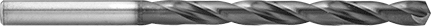
\includegraphics[width=0.95\textwidth]{imgs/drillbit.png}
		\caption{Drillbit}
	\end{subfigure} \begin{subfigure}[b]{.19\linewidth}
		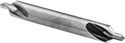
\includegraphics[width=0.95\textwidth]{imgs/centerdrill.png}
		\caption{Centerdrill}
	\end{subfigure}	\begin{subfigure}[b]{.19\linewidth}
		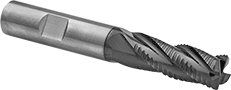
\includegraphics[width=0.95\textwidth]{imgs/endmill.png}
		\caption{End mill}
	\end{subfigure}	\begin{subfigure}[b]{.19\linewidth}
		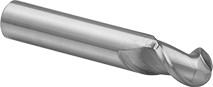
\includegraphics[width=0.95\textwidth]{imgs/ball_endmill.png}
		\caption{Ball end mill}
	\end{subfigure}\begin{subfigure}[b]{.19\linewidth}
		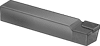
\includegraphics[width=0.95\textwidth]{imgs/lathetool.png}
		\caption{Lathe tooling}
	\end{subfigure}	
	
	\caption{Machine Tooling}
\end{figure}

 \begin{asparaenum}[a)]
 	\item \textit{Drillbits} drill holes. The spiral flutes on the outside may be sharp, but they generally aren't sharp or hard enough to actually cut metal. They work with jacobs chucks, which are designed to only transmit vertical force and torque.
 	\item \textit{Centerdrills} are used to start holes. They are short and stubby, so don't deflect much.
 	\item \textit{End mills} cut on all surfaces- they are all ground to be sharp and cut. This means they can cut on the side, and produce side loads- so they should not be put in jacobs chucks in drill presses!
 	\item \textit{Ball end mills} are an example of a more sophisticated end mill. There are many different shapes. This one enables smooth contours to be made.
 	\item \textit{Lathe tooling} comes in many different shapes and sizes. This one is a simple cutting tool that gets clamped to the toolpost and shapes the outside of the work.
 \end{asparaenum}
 
If you can consider briefly how these machines work, you can perhaps spot a few problems with your designs as you go along. Can you spot (just by the images) some issues with these parts?
 
\begin{figure}[H]
	\centering
	\begin{subfigure}[b]{.24\linewidth}
		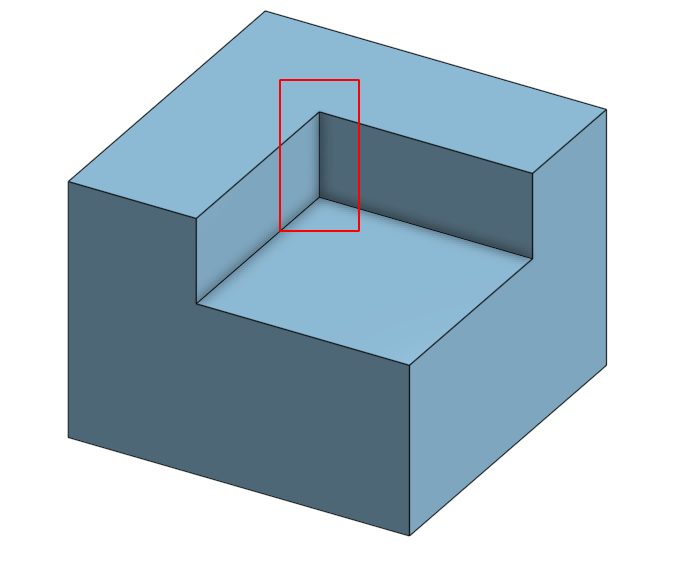
\includegraphics[width=0.9\textwidth]{imgs/nonmill_sharpins.png}
		\caption{Sharp inside corner}
	\end{subfigure}	\begin{subfigure}[b]{.24\linewidth}
		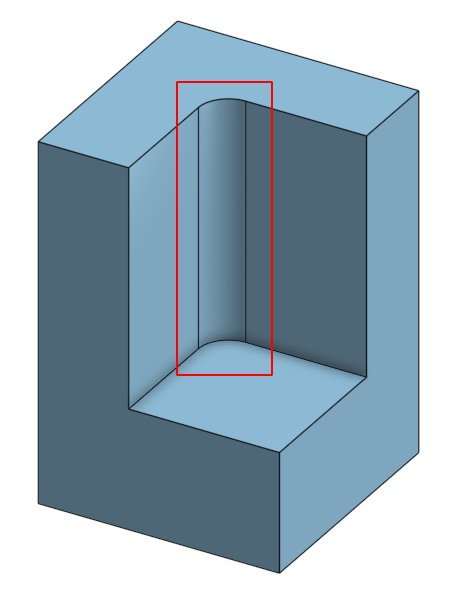
\includegraphics[width=0.9\textwidth]{imgs/nonmill_dtod.png}
		\caption{Deep radius}
	\end{subfigure}	
	
	\caption{Problematic geometries for machining}
\end{figure}

 \begin{asparaenum}[a)]
 	\item The sharp inside corner cannot be made, as it would require an infinitely small diameter tool.
 	\item The deep radius would require a very long end mill, which would not be very stiff. This radius is 0.25", and it is 2" tall; this is a ratio of depth-to-diameter of 4:1, which is a suboptimal ratio. Ideally, this ratio would be no more than 3:1.
 \end{asparaenum}
 
 \subsection{Broaching}
 
 
 \begin{figure}[H]
 	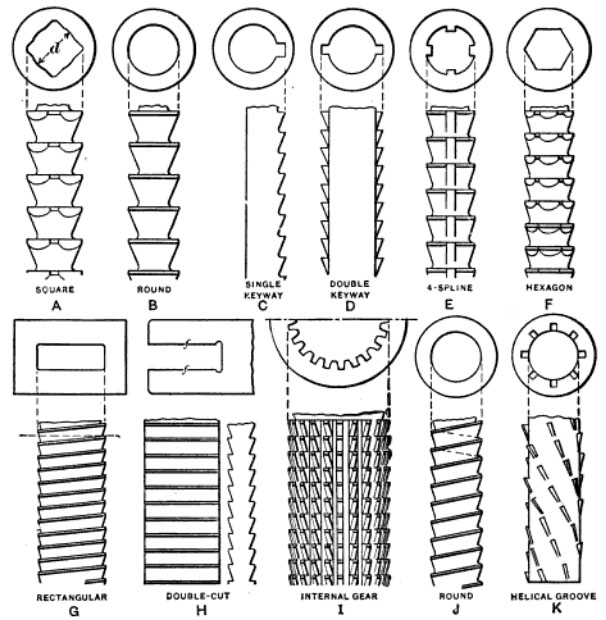
\includegraphics[width=0.6\textwidth]{imgs/broach_examples.jpeg}
 	\caption{Broach Examples}
 \end{figure}
 
 But how do we make splines, keyways, and hexes in things? Those need infinitely sharp corners, so we broach them. This is done by first drilling a hole of the appropriate diameter, and then inserting a broaching tool into the hole. The tool is then pushed through with a press. Each tooth of the broach takes off gradually more material until the final shape is achieved. Broaches are typically very expensive and relatively delicate tools.
 
 \begin{figure}[H]
 	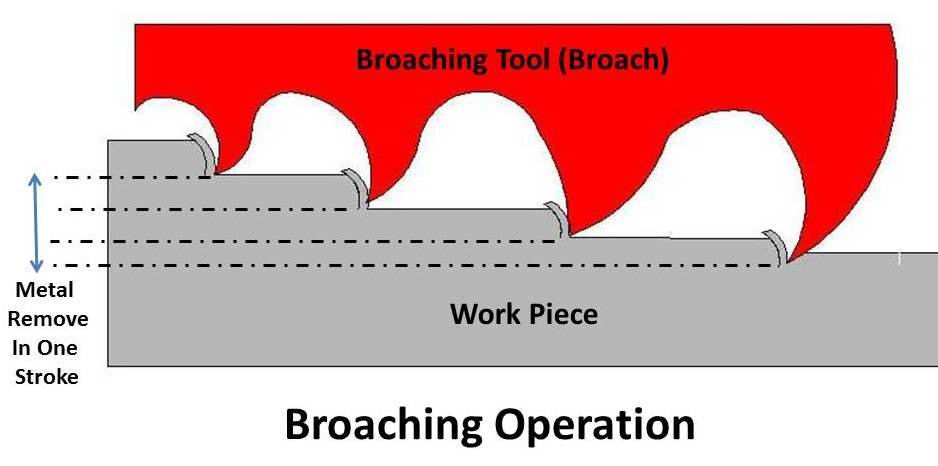
\includegraphics[width=0.7\textwidth]{imgs/broach_detail.jpeg}
 	\caption{Broach Detail}
 \end{figure}
 
 
 \subsection{Path Cutting}
 
 \textit{Path cutting} is a term I made up that encompasses any sort of 2-dimensional X/Y cutting with a thin beam. It is almost always done on a CNC-capable machine.
 
 \begin{figure}[H]
		\begin{subfigure}[b]{.24\linewidth}
			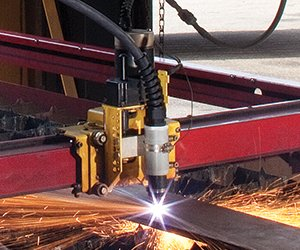
\includegraphics[width=0.9\textwidth]{imgs/plasmacut.jpeg}
			\caption{Plasma cutting}
		\end{subfigure}\begin{subfigure}[b]{.24\linewidth}
			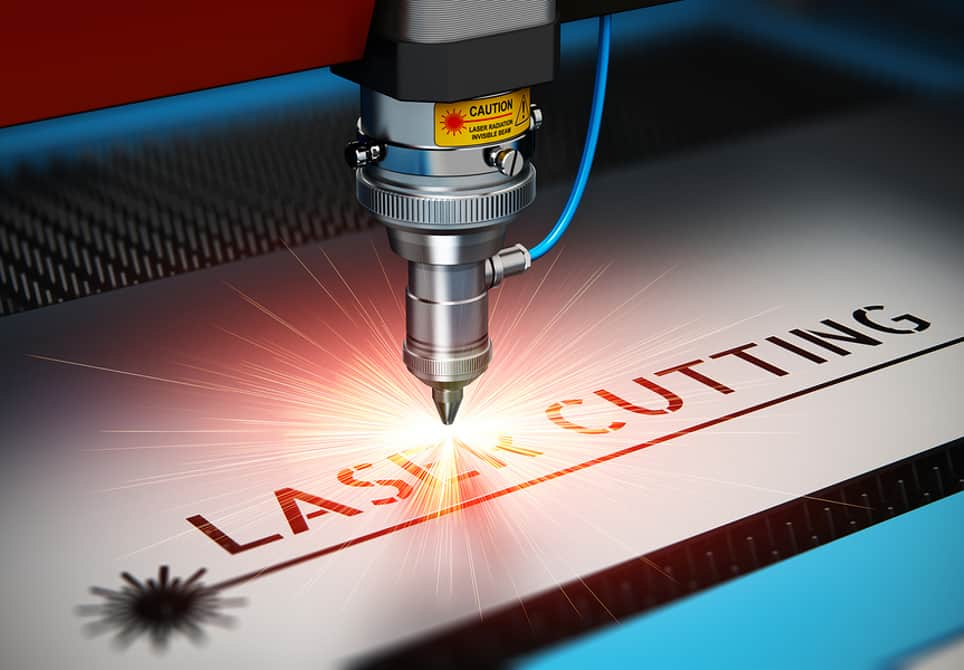
\includegraphics[width=0.9\textwidth]{imgs/lasercut.jpeg}
			\caption{Laser cutting}
		\end{subfigure}\begin{subfigure}[b]{.24\linewidth}
			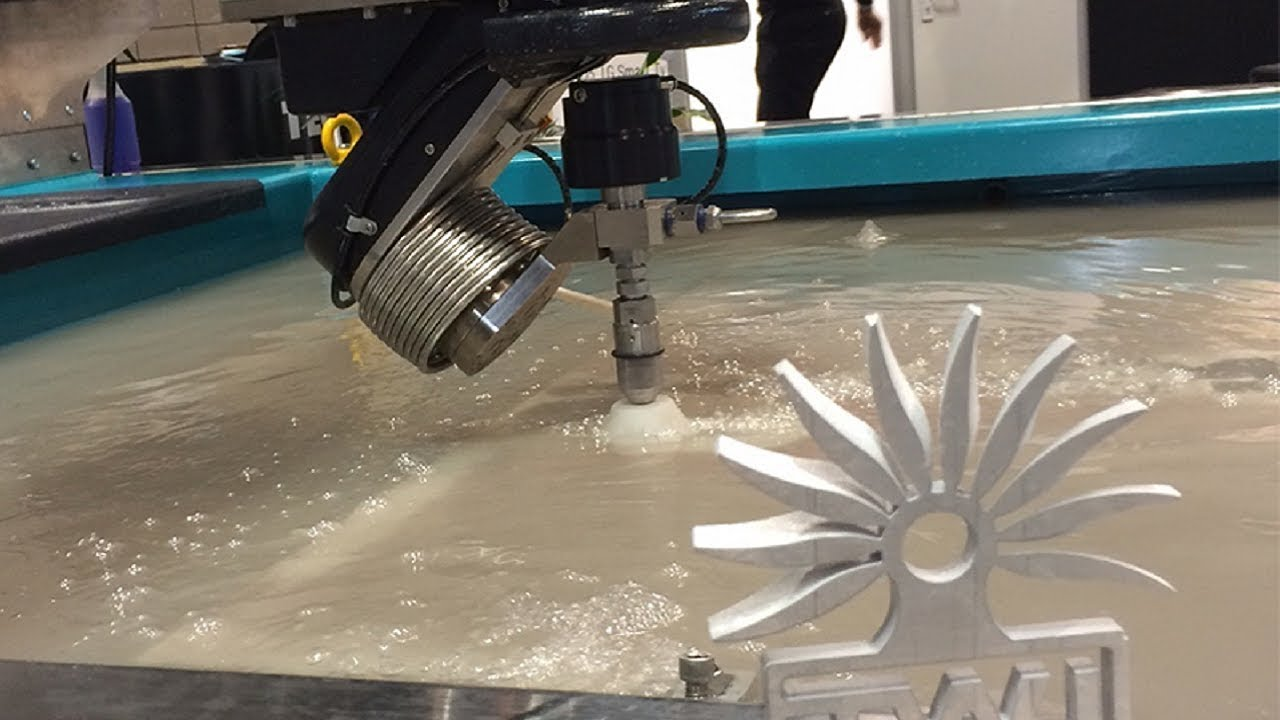
\includegraphics[width=0.9\textwidth]{imgs/waterjet.jpeg}
			\caption{Waterjet cutting}
		\end{subfigure}\begin{subfigure}[b]{.24\linewidth}
			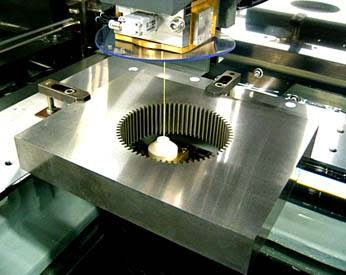
\includegraphics[width=0.9\textwidth]{imgs/edm.jpeg}
			\caption{EDM cutting}
		\end{subfigure}
	\end{figure}
 
 \begin{asparaenum}[a)]
  	\item \textit{Plasma cutters} use an arc to melt metal and pressurized air to blow it away. The tolerances are usually good for large shapes, but not for precision work.
 	\item \textit{Laser cutters} melt material with a laser and either simply vaporize it or use pressurized air to blow it away. Hobby lasers can cut some plastics and plywood, while industrial systems can cut metal. The tolerances are usually acceptable with these machines ($\pm 0.020"$).
 	\item \textit{Waterjet cutters} mix high-pressure water with garnet sand, and blast it at material, rapidly abrading it. The tolerances are usually good with this process ($\pm 0.010"$ or better).
 	\item \textit{EDMs} (electro-discharge-machines) use an electrified wire to remove material. The wire is fed through (or plunged into) material. The electrification 'zaps' away material next to the wire. The tolerances with this process can be impeccable ($\pm 0.001"$ or better). 
\end{asparaenum}
 	
 	These all allow us to overcome the depth-to-diamter ratio imposed by milling, and can sometimes be much quicker setup than traditional machining, though they all come with their own drawbacks.
 
 \begin{figure}[H] \centering
 	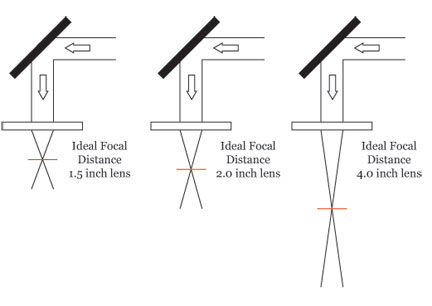
\includegraphics[width=0.5\textwidth]{imgs/lasercut_focus.jpeg}
 	\caption{Focal properties of a lasercutter's beam.}
 \end{figure}
 
  The first limitation is the width of the beam. Since a finite-ly sized beam muse be used, infinitely sharp interior corners cannot be made.
 
 \begin{figure}[H] \centering
 	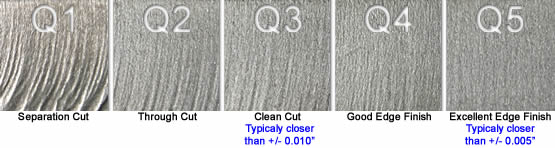
\includegraphics[width=0.9\textwidth]{imgs/waterjet_draft.jpeg}
 	\caption{Draft and surface quality samples on a waterjet with different settings.}
 \end{figure}
 
  The next consideration that must be made is draft. Laser-cutters typically have a point in the thickness where the beam is focused to. This means that the laser doesn't cut a line in its cross-section, but rather an X. Thus the resulting shape is two-dimensional. With a waterjet or plasma cutter, the draft grows exponentially. This may be acceptable, or require further post-machining to bring it into specification.
 
 Draft (and power) also limits how thick of material can feasibly be cut with these processes, although EDM can cut extremely thick materials compared to the other processes.
 
 \subsection{Sheet Forming}
 
 Sheet forming is a versatile process of making parts from, well, sheet. Sheet may be cut either with a stamping operation, or with a path-cutting operation to form a blank. This blank can then be loaded in and undergo one of several processes.
 
 	\begin{figure}[H]
		\centering
		\begin{subfigure}[b]{.24\linewidth}
			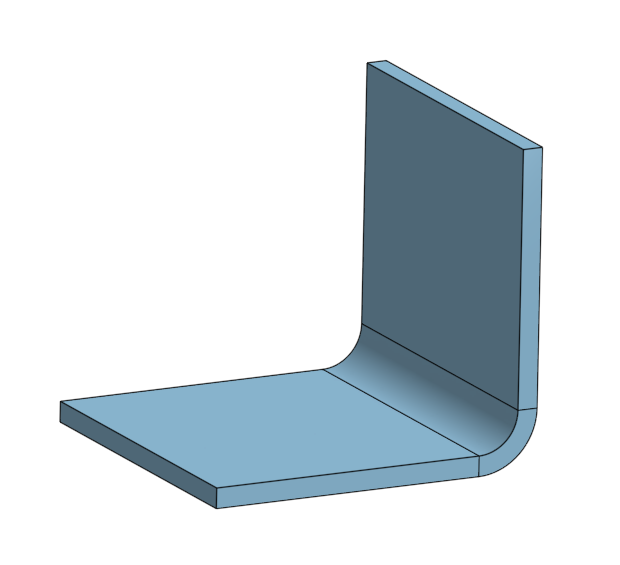
\includegraphics[width=0.9\textwidth]{imgs/sheet_bend.png}
			\caption{Bend}
		\end{subfigure}\begin{subfigure}[b]{.24\linewidth}
			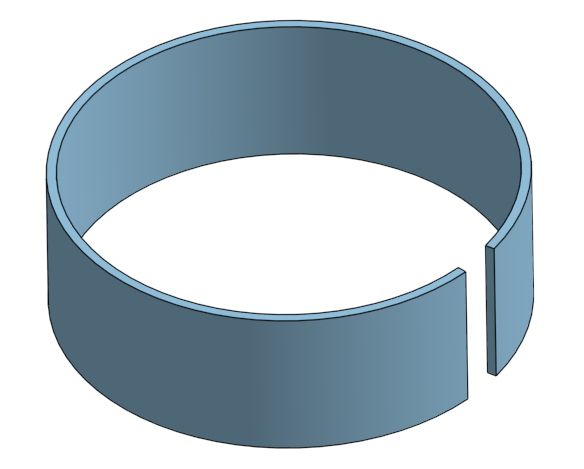
\includegraphics[width=0.9\textwidth]{imgs/sheet_roll.png}
			\caption{Rolling}
		\end{subfigure}\begin{subfigure}[b]{.24\linewidth}
			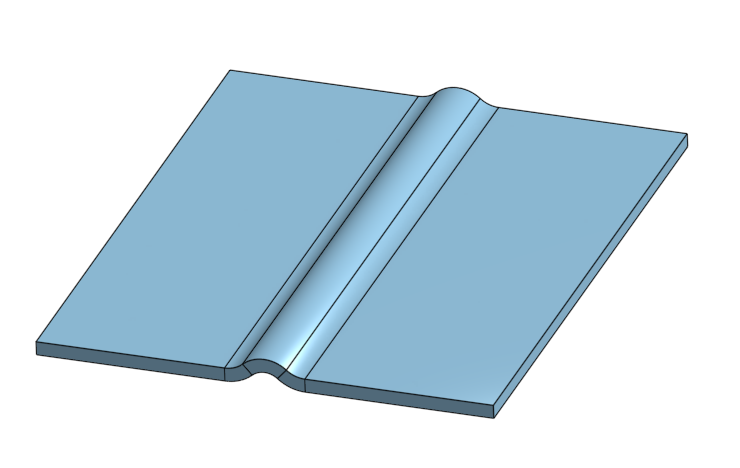
\includegraphics[width=0.9\textwidth]{imgs/sheet_beadroll.png}
			\caption{Bead Rolling}
		\end{subfigure}\begin{subfigure}[b]{.24\linewidth}
			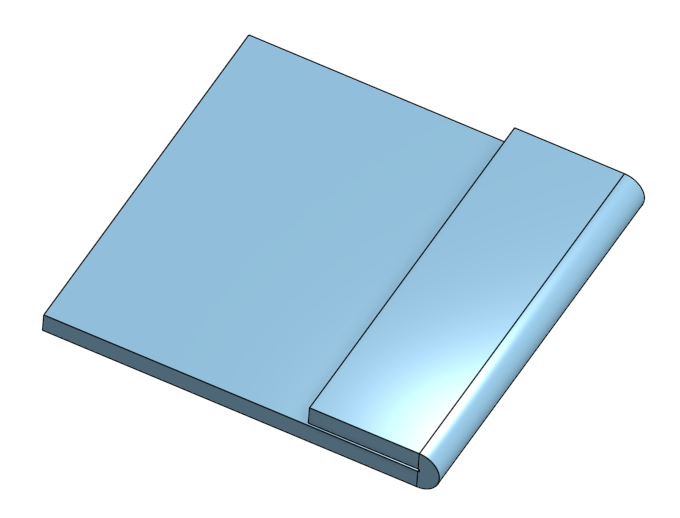
\includegraphics[width=0.9\textwidth]{imgs/sheet_hem.png}
			\caption{Hemming}
		\end{subfigure}
		\caption{Rudimentary sheetmetal operations.}
	\end{figure} 
 
 \begin{asparaenum}[a)]
 	\item Simple \textit{bends} can be made on a linear portion of the flat pattern. This can be done with a finger bender, press brake, or (in a pinch) a vise with a hammer.
 	\item Flat portions of material can be \textit{rolled} into an arc, or even full circle.
 	\item \textit{Bead rolling} can be done on any portion of a part to provide additional stiffness.	
 	\item \textit{Hemming} provides a smooth, radiused outer corner and some additional stiffness. First, a bend is made, and then it is bent all the way to 180 degrees. This can be done with a finger bender or press brake, and additional clamping to finish the hem.
 	\end{asparaenum}
 	
 	Most CAD packages have tools to design parts made with sheetmetal. You can draw up the bent part, and then the CAD package will determine how to 'unfold' and produce a flat pattern that can be cut out.
 	
 	These operations are typically done with metal, but nothing prevents you from doing it with plastic. Polycarbonate can be bent like sheetmetal. Polypropylene, polycarbonate, acrylic, and PETG amongst others can also be heated (i.e. with a heat gun) and then bent by hand.
 	
 	\subsection{Welding and Brazing}
 	
 	Welding and brazing are very important manufacturing methods. They enable large, complex structures to be made from smaller simple ones, without fasteners that might fail. However, it can be quite time consuming, requires time consuming labor, and creates non-servicable structures.
 	
 	\begin{figure}[H]
		\centering
		\begin{subfigure}[b]{.24\linewidth}
			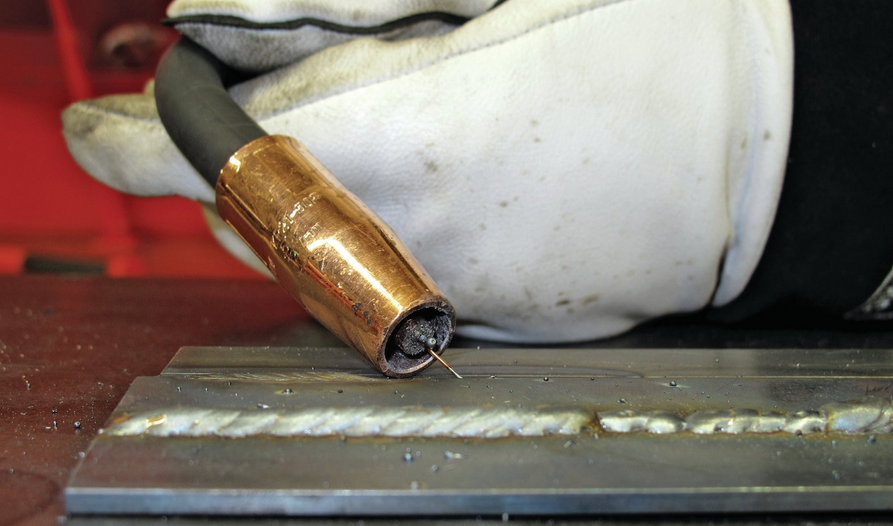
\includegraphics[width=0.9\textwidth]{imgs/mig.png}
			\caption{MIG}
		\end{subfigure}\begin{subfigure}[b]{.24\linewidth}
			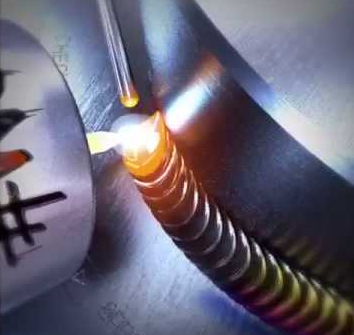
\includegraphics[width=0.9\textwidth]{imgs/tig.png}
			\caption{TIG}
		\end{subfigure}\begin{subfigure}[b]{.24\linewidth}
			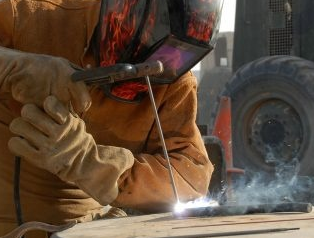
\includegraphics[width=0.9\textwidth]{imgs/arcweld.png}
			\caption{Stick/Arc Welding}
		\end{subfigure}\begin{subfigure}[b]{.24\linewidth}
			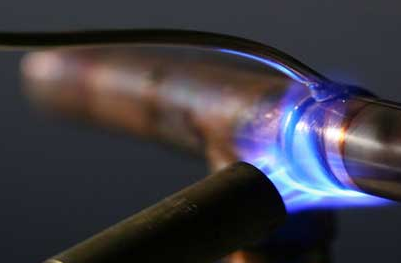
\includegraphics[width=0.9\textwidth]{imgs/braze.png}
			\caption{Brazing}
		\end{subfigure}
		\caption{Various welding/brazing technologies.}
	\end{figure}
 	
 	\begin{asparaenum}[a)]
 		\item \textit{MIG} (Metal-Inert-Gas) welding uses an electric arc between filler wire and the workpiece, which melts both the wire and the workpiece. The arc is shielded by inert (or semi-active) gas to control chemical reactions. The wire is advanced at a constant rate into the workpiece. This is the easiest method to learn, but provides the least amount of control, and has the lowest capacity for superior results.
 		
 		\item \textit{TIG} (Tungsten-Inert-Gas) welding uses an electric arc between a fixed tungsten rod and the workpiece, melting the work but not the tungsten. The arc is shielded by inert gas to eliminate chemical reactions. Filler rod is advanced manually and separately into the molten work. This method is much harder to learn, but provides the most amount of control, with the highest capacity for superior results.
 		
 		\item \textit{Stick} (or Arc) welding uses an electric arc between a rod containing flux and filler metal and the workpiece, melting both the rod and the workpiece.. The arc is shielded by the vaporizing flux. This method is hard to learn, but provides good control, and works best outdoors, so is quite common in the construction and pipeline industries.
 		
 		\item In \textit{brazing}, heat is generated (either by a TIG torch, or a flame torch) and directed at the work, but not enough to melt the work. Brazing material, which will melt at this surface temperature, is fed onto the work, melting and flowing across it. As it solidifies, it adheres to the base metal.
 		
 	\end{asparaenum}
 		
	\section{Fasteners}
	So you've made some parts, now it's time to put them together. How are you going to do it? CAD constraints won't help you now! You need real fasteners!
	
	\subsection{Pins}
	The simplest fastener is a pin. Pins prevent holes in plates from shearing past each other, by putting all of the load through the pin. There are a couple different flavors that let you do different things.
	
	Quick pins allow users to easily make adjustments or reconfigurations to equipment. They are easily insertable/removable, usually without any special tools.
	
	\begin{figure}[H]
		\centering
		\begin{subfigure}[b]{.32\linewidth}
			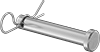
\includegraphics[width=0.7\textwidth]{imgs/cpin.png}
			\caption{Clevis pin}
		\end{subfigure}\begin{subfigure}[b]{.32\linewidth}
			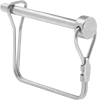
\includegraphics[width=0.7\textwidth]{imgs/wlpin.png}
			\caption{Wire-locking pin}
		\end{subfigure}\begin{subfigure}[b]{.32\linewidth}
			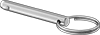
\includegraphics[width=0.7\textwidth]{imgs/bdpin.png}
			\caption{Ball-detent pin}
		\end{subfigure}
		\caption{Various quick-removal pins.}
	\end{figure}
	
	\begin{asparaenum}[a)]
		\item \textit{Clevis pins} are loose tolerance pins which have a hole for a locking (R-shaped) pin or wire to go through.
		\item \textit{Wire-Locking pins} serve the same purpose as clevis pins, but use a spring-loaded wire to keep the pin captive.
		\item \textit{Ball-Detent pins} serve the same purpose as clevis pins, but use a spring-loaded ball detent to keep the pin captive. These can be pulled/pushed in without and additional steps.
	\end{asparaenum}
	
	
	Precision pins serve a nearly opposite purpose- they are permanent instalations, but provide extremely tight tolerances when used right. They allow for installation/detachment of components with high repeatability in locational positioning. It's not uncommon to see precision equipment register together with pins, and then be bolted together in addition to the pins. Pins also can provide higher load transferral since they do not have the stress concentrators that bolts do.
	
	\begin{figure}[H]
		\centering
		\begin{subfigure}[b]{.24\linewidth}
			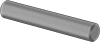
\includegraphics[width=0.7\textwidth]{imgs/dpin.png}
			\caption{Dowel pin}
		\end{subfigure}\begin{subfigure}[b]{.24\linewidth}
			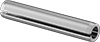
\includegraphics[width=0.7\textwidth]{imgs/spin.png}
			\caption{Spring pin}
		\end{subfigure}\begin{subfigure}[b]{.24\linewidth}
			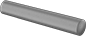
\includegraphics[width=0.7\textwidth]{imgs/tpin.png}
			\caption{Taper pin}
		\end{subfigure}\begin{subfigure}[b]{.24\linewidth}
			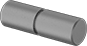
\includegraphics[width=0.7\textwidth]{imgs/shpin.png}
			\caption{Shear pin}
		\end{subfigure}
		\caption{Various precision pins.}
	\end{figure}
	
	\begin{asparaenum}[a)]
		\item \textit{Dowel pins} are tight-tolerance. They are typically pressed into one part's hole, and with a loose fit on another mating part.
		\item \textit{Spring pins} are formed from coiled metal, intended to be pressed in like a dowel pin, but have some give to them so can be used with looser-tolerance holes.
		\item \textit{Taper/scotch pins} are like dowel pins, but they are slightly tapered, so they wedge into multiple parts like a nail.
		\item \textit{Shear pins} are specifically designed to fail at a specified load, which prevents damage to equipment down-the-line.
	\end{asparaenum}
	
	\subsection{Threads}
	
	Threaded fasteners (bolts, nuts, and screws) are a ubiquitous solution. There's an age old question of what is a 'screw' versus a 'bolt' and the answer is merely in application- if it goes into a nut, it's a bolt. Otherwise, it's a screw. So, anything said about screws is true of bolts and vise-versa.
	
	\begin{figure}[H]
		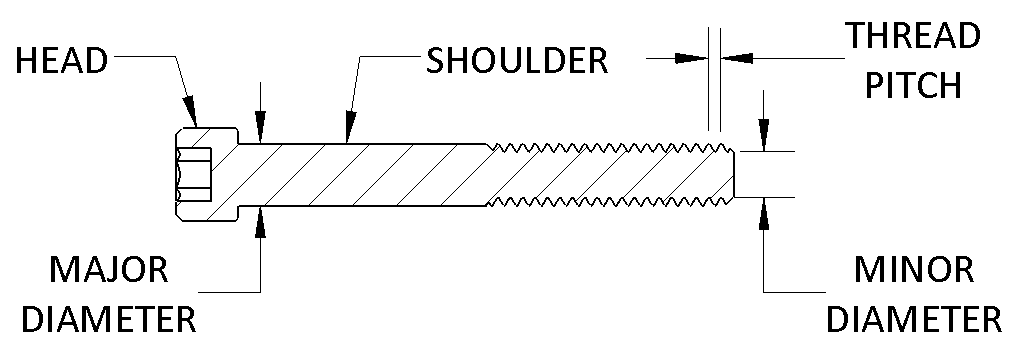
\includegraphics[width=0.7\textwidth]{imgs/thread_nomenclature.png}
		\caption{Thread nomenclature and dimensions.}
	\end{figure}
	
	Threaded fasteners are denoted by:
	\begin{asparaitem}
		\item The major diameter of the thread.
		\item The thread pitch, or threads-per-inch. Metric bolts are specced by the pitch (a M5x0.8 has 0.8mm between each thread crest). English bolts are specced by the number of thread crests in an inch (a 1/4"-20 has 20 threads per inch, or a pitch of 1/20 = 0.05 inches). Even among the same diameter, bolts can have different pitches. For instance, a 1/4"-28 is fine thread, and a 1/4"-20 is coarse thread.
		\item The thread length - the bolt might be threaded fully, or only partially. The unthreaded portion is the shoulder and is usually the same diameter as the threads' major diameter.
		\item The handedness of the thread - most threads are right handed (meaning turning them in a clockwise fashion will make them move away) unless specified as left-handed.
		\item The grade or class - this refers to the strength of the material. English bolts are specified by "grade", and metric bolts by "class". Bolts (usually) have head markings that reflect the material. Grade and class are only for steel, though- other materials have more exotic standards.
	\end{asparaitem}
	
	There are many different types of bolts out there.
	
	\begin{figure}[H]
		\centering
		\begin{subfigure}[b]{.24\linewidth}
			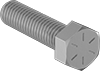
\includegraphics[width=0.7\textwidth]{imgs/hhcs.png}
			\caption{External drive}
		\end{subfigure}\begin{subfigure}[b]{.24\linewidth}
			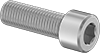
\includegraphics[width=0.7\textwidth]{imgs/shcs.png}
			\caption{Socket head}
		\end{subfigure}\begin{subfigure}[b]{.24\linewidth}
			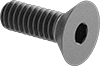
\includegraphics[width=0.7\textwidth]{imgs/fhcs.png}
			\caption{Flathead}
		\end{subfigure}\begin{subfigure}[b]{.24\linewidth}
			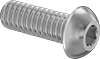
\includegraphics[width=0.7\textwidth]{imgs/bhcs.png}
			\caption{Button head}
		\end{subfigure}
		
		\begin{subfigure}[b]{.24\linewidth}
			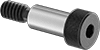
\includegraphics[width=0.7\textwidth]{imgs/shoulderscrew.png}
			\caption{Shoulder screw}
		\end{subfigure}\begin{subfigure}[b]{.24\linewidth}
			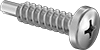
\includegraphics[width=0.7\textwidth]{imgs/stscrew.png}
			\caption{Self-tapping screw}
		\end{subfigure}\begin{subfigure}[b]{.24\linewidth}
			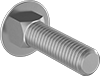
\includegraphics[width=0.7\textwidth]{imgs/carriagebolt.png}
			\caption{Carriage bolt}
		\end{subfigure}\begin{subfigure}[b]{.24\linewidth}
			\includegraphics[width=0.7\textwidth]{imgs/grubscrew.png}
			\caption{Grub or set screw}
		\end{subfigure}
		\caption{Various screws / bolts.}
	\end{figure}
	
	\begin{asparaenum}[a)]
		\item \textit{External drive} bolts are good when only side-access is possible, or a cheap solution is needed. The most common example is a hex-head bolt, though pentagon-, external-torx-, and square- heads exist.
		\item \textit{Socket head} bolts are preferred. They can be installed in deep wells and have a compact head profile.
		\item \textit{Flat head} screws need to be installed into holes that have been countersunk to the same angle as the head of the screw. They allow for a flush, smooth installation. However, they have a smaller hex than socket heads of the same thread diameter. This makes them more prone to stripping the head out.
		\item \textit{Button head} screws provide a smooth surface without the need to countersink the surface. They still have a smaller-diameter hex than socket-heads, though, so are generally unpreferred.
		\item \textit{Shoulder screws} are special-use screws. The shoulder (unthreaded) portion is precision ground and usually a larger diameter than the thread. This allos them to be used as pins or pivot points.
		\item \textit{Self-tapping screws} have specially formed tips based on what material they are designed to tap into. They thread into material directly; a tap is not required to form threads, and in plastic and wood, are generally stronger.
		\item \textit{Carriage bolts} have a rounded head without any means of being driven externally. Instead, the square portion sitting under the thread mates with the material it bolts together (either a plate with the corresponding female portion, or a soft material like wood conforms to the square). \textit{Plow bolts} are the same principle, but are flat-headed.
		\item \textit{Set screws} (often called \textit{grub screws}) are used to lock down on another piece of material. Commonly seen to secure hubs to shafts. They have very small hexes relative to their thread diameter and are notorious for stripping out.
	\end{asparaenum}
	
	There are a lot of different head types that can be put on these bolts as well. 
	
	\begin{figure}[H]
		\centering
		\begin{subfigure}[b]{.15\linewidth}
			\includegraphics[width=0.7\textwidth]{imgs/head_ext_hex.png}
			\caption{External hex}
		\end{subfigure}\begin{subfigure}[b]{.15\linewidth}
			\includegraphics[width=0.7\textwidth]{imgs/head_hex.png}
			\caption{Socket hex}
		\end{subfigure}\begin{subfigure}[b]{.15\linewidth}
			\includegraphics[width=0.7\textwidth]{imgs/head_slot.png}
			\caption{Flathead}
		\end{subfigure}\begin{subfigure}[b]{.15\linewidth}
			\includegraphics[width=0.7\textwidth]{imgs/head_phil.png}
			\caption{Phillips}
		\end{subfigure}\begin{subfigure}[b]{.15\linewidth}
			\includegraphics[width=0.7\textwidth]{imgs/head_torx.png}
			\caption{Torx}
		\end{subfigure}\begin{subfigure}[b]{.15\linewidth}
			\includegraphics[width=0.7\textwidth]{imgs/head_robertson.png}
			\caption{Robertson}
		\end{subfigure}
		\caption{Common drive types on engineering fasteners.}
	\end{figure}
	
	\begin{asparaenum}[a)]
		\item \textit{External hex} is very robust, although prefferred only when side access is available as it has a large profile.
		\item \textit{Socket hex} has become an industry preferred head, very easy to access from head-on or in a deep pocket.
		\item \textit{Flathead} is an unpreferred drive type; it is very easy to have driver fall out while using, and the torque-transferring capacity is quite low.
		\item \textit{Phillips} heads are very much unpreferred as they are very easy to cam out (in fact, they were designed to do so as a means of limiting the installation torque). When driving a phillips screw, apply inward pressure, and make sure the proper size driver is selected (it should fit nicely).
		\item \textit{Torx} is a preferred drive method, but more expensive and the tools to use it are less common. Very difficult to strip out. When using button-head or flat-head screws, if a torx variant is available, it can be wise to opt for it as the torque-transferring capacity is higher.
		\item \textit{Robertson} or square drive is somewhat preferred, but not common. Usually found only in wood screws.
	\end{asparaenum}
	
	
	\begin{figure}[H]
		\includegraphics[width=0.5\textwidth]{imgs/bolt_preload.png}
		\caption{Aspects of a bolted joint.}
		 \label{fig:bolted_joint} 
	\end{figure}
	
	When you tighten a screw to a torque, this not only prevents the nut from falling off, but clamps the parts together. This clamping force that is imparted upon installation is \textit{preload}. Preload is very important in threaded joints. For shear loads as illustrated in Figure \ref{fig:bolted_joint}, the load is best carried by the friction inbetween plates rather than shearing the pin itself, since the load is distributed across a larger area. For joints that seal against pressures, preload is imperative as it prevents separation under pressure.
	
	The preload depends both on how much torque is applied to the fastener, and the pitch of the thread. A finer-pitched screw will impart greater preload. Finer-pitched screws also have the benefit of an increased core (minor) diameter, so greater strength in shear.
	
	Spreading the load across the greater area increases rigidity and decreases backlash, egg-out, and strength. However, too much torque can dig the head of the bolt/screw into the underlying material, especially if it is soft (like plastic, or even aluminum). As such, care not to overtorque, or a washer may be needed.
	
	\begin{figure}[H]
		\centering
		\begin{subfigure}[b]{.24\linewidth}
			\includegraphics[width=0.7\textwidth]{imgs/plainwasher.png}
			\caption{Plain washer}
		\end{subfigure}\begin{subfigure}[b]{.24\linewidth}
			\includegraphics[width=0.7\textwidth]{imgs/machinewasher.png}
			\caption{Machine washer}
		\end{subfigure}\begin{subfigure}[b]{.24\linewidth}
			\includegraphics[width=0.7\textwidth]{imgs/fenderwasher.png}
			\caption{Fender washer}
		\end{subfigure}
		\caption{Plain washers of differring sizes}
	\end{figure}
	
	Bolts thread into nuts, which can be replaced if they strip out. But if the material a screw threads into strips, then that whole piece will need to be replaced or repaired- which can be even more costly. There are some considerations that can be made to ensure success when using integral threads. The first is to make sure to use coarse (not fine) threads in soft materials like aluminum or plastic. Another option is to use thread inserts.
	
	\begin{figure}[H]
		\centering
		\begin{subfigure}[b]{.24\linewidth}
			\includegraphics[width=0.5\textwidth]{imgs/helicoil.png}
			\caption{Helicoil}
		\end{subfigure}\begin{subfigure}[b]{.24\linewidth}
			\includegraphics[width=0.5\textwidth]{imgs/tanglock.png}
			\caption{Tang-lock insert}
		\end{subfigure}\begin{subfigure}[b]{.24\linewidth}
			\includegraphics[width=0.5\textwidth]{imgs/rivnut.png}
			\caption{Rivnut}
		\end{subfigure}\begin{subfigure}[b]{.24\linewidth}
			\includegraphics[width=0.5\textwidth]{imgs/pemnut.png}
			\caption{PEM nut}
		\end{subfigure}
		
		\begin{subfigure}[b]{.24\linewidth}
			\includegraphics[width=0.5\textwidth]{imgs/heatset.png}
			\caption{Heat-set insert}
		\end{subfigure}\begin{subfigure}[b]{.24\linewidth}
			\includegraphics[width=0.5\textwidth]{imgs/teenut.png}
			\caption{Tee nut}
		\end{subfigure}\begin{subfigure}[b]{.24\linewidth}
			\includegraphics[width=0.5\textwidth]{imgs/woodsti.png}
			\caption{Wood tapping insert}
		\end{subfigure}
		\caption{Various threaded inserts}
	\end{figure}
	
	\begin{asparaenum}[a)]
		\item \textit{Helicoils} can be installed after a thread strips out, or before it does preventatively. They are a coiled piece of metal formed like threads.
		\item \textit{Tang-lock inserts} work much like helicoils, but are solid-bodied rather than coiled, and have locking tangs that can be hammered down on installation to make sure the insert doesn't back out.
		\item \textit{Rivnuts} (rivet nuts) can be installed into holes in thin metal to provide ample threads for fastening. They work much like rivets (more on those later), but need a special tool.
		\item \textit{PEM nuts} serve the same purpose as rivnuts, but are simply pressed into the sheet they are to be installed in.
		\item \textit{Heat-set inserts} are for plastic. They are instaled by heating them up with a soldering iron and pressing them into thermoplastic. An excellent addition to 3D prints.
		\item \textit{Tee nuts} are meant to be pressed into wood, much like a PEM nut. The large flange prevents tear-out and helps distribute load in soft wood.
		\item \textit{Wood tapping inserts} are much like tang-lock inserts, but with larger wings suitable for wood.
	\end{asparaenum}
	
	Threaded joints have one big weakness, and that is their subsceptibility to vibration. There are many solutions to try and combat this.
	
	\begin{figure}[H]
		\centering
		\begin{subfigure}[b]{.24\linewidth}
			\includegraphics[width=0.8\textwidth]{imgs/lockwire.png}
			\caption{Safety/lock wire}
		\end{subfigure}\begin{subfigure}[b]{.24\linewidth}
			\includegraphics[width=0.8\textwidth]{imgs/threadlocker.jpeg}
			\caption{Threadlocker}
		\end{subfigure}\begin{subfigure}[b]{.24\linewidth}
			\includegraphics[width=0.5\textwidth]{imgs/nylock.png}
			\caption{Nylock nut}
		\end{subfigure}\begin{subfigure}[b]{.24\linewidth}
			\includegraphics[width=0.7\textwidth]{imgs/kaynut.png}
			\caption{Kay/jet nut}
		\end{subfigure}
		
		\begin{subfigure}[b]{.24\linewidth}
			\includegraphics[width=0.5\textwidth]{imgs/jamnut.png}
			\caption{Jam nut}
		\end{subfigure}\begin{subfigure}[b]{.24\linewidth}
			\includegraphics[width=0.5\textwidth]{imgs/nordlock.png}
			\caption{Nordlock washer}
		\end{subfigure}\begin{subfigure}[b]{.24\linewidth}
			\includegraphics[width=0.5\textwidth]{imgs/splitlock.png}
			\caption{Split lock washer}
		\end{subfigure}\begin{subfigure}[b]{.24\linewidth}
			\includegraphics[width=0.5\textwidth]{imgs/castlenut.png}
			\caption{Castle nut}
		\end{subfigure}
		\caption{Thread locking strategies.}
	\end{figure}
	
	\begin{asparaenum}[a)]
		\item Lock wire requires tedious installation and bolts with cross-drilled holes to feed the stainless steel wire through. That said, when it is installed properly, it is virtually failure-proof, and as such is the standard in many aerospace and motorsport applications. 
		\item Threadlocker (sometimes referred to by the brand name Loctite) comes in various different strengths and can be used on metal-on-metal contact. It's basically long-cure, specially formulated superglue. However, it does attack many plastics, so be careful! It also requires time to cure to full strength, so is not an instant fix, but must be premeditated.
		\item Nylock nuts have a nylon patch that deforms when the threads pass through it. The nut should be installed metal-side first, nylon-side last. These are limited use (<50 uses).
		\item Kay/Jet nuts (metal locknuts) work on the same idea as nylock nuts, but in this case, the nut is deformed and interferes with the thread. It is quite difficult to thread into these nuts. These are extremely limited use (<5 uses) but will work in extreme temperatures, unlike nylocks.
		\item Jam Nuts are simply a second nut jammed up against the first nut. This enables easy adjustment, but is not a very positive way of locking something in place.
		\item Nordlock washers are special ratcheting washers which prevent loosening when properly torqued. There are many different types of locking washers.
		\item Split lock washers are cheap washers which arguably do not actually prevent loosening.
		\item Castle nuts are nuts with slots through which a pin can be fed, locking the nut to the bolt it is secured to. A very robust method.
	\end{asparaenum}
	
	\subsection{Rivets}
	
	Pop rivets are a light and cheap method of fastening. However, they require a special gun and are one-time use. They must be drilled out in order to remove them. They are weaker than bolts, so more must be used, but overall, they are a lighter option. Installation is also more picky than bolting. However, they can still be a time-saver over bolts (when disassembly is not a factor).
	
	Rivets are specified by diameter and 'grip length'; the amount of material sandwiched together they can grip. Rivets should be installed to close-fit holes, straight, and with the plates already pulled together.
	
	\begin{figure}[H] \centering
		\includegraphics[width=0.9\textwidth]{imgs/rivet_install.jpeg}
		\caption{Left: Process of Rivet Installation. Right: Diagnosing rivet failures.}
	\end{figure}
	
	Hot rivets are a very different animal than pop rivets. These require very specialized equipment, and work by heating up a rivet to molten temperature, inserting it through the hole to be secured, and hammering it so it expands and mushrooms out on both sides. As the rivet cools, it shrinks further, creating an incredibly robust and secure connection.	
	
	\subsection{Shaft Retention}
	
	Retaining rings are used to constrain objects along a shaft.
	
	\begin{figure}[H]
		\centering
		\includegraphics[width=0.45\textwidth]{imgs/shaft_snapringgroove.png}
		\includegraphics[width=0.45\textwidth]{imgs/snapringtool.jpeg}
		\caption{Left: Shaft with groove for retaining ring. Right: Snap ring pliers.}
	\end{figure}
	
	\begin{figure}[H]
		\centering
		\begin{subfigure}[b]{.24\linewidth}
			\includegraphics[width=0.6\textwidth]{imgs/shaftcollar.png}
			\caption{Shaft collar}
		\end{subfigure}
		\begin{subfigure}[b]{.24\linewidth}
			\includegraphics[width=0.7\textwidth]{imgs/pushonring.png}
			\caption{Push-on ring}
		\end{subfigure}
		\begin{subfigure}[b]{.24\linewidth}
			\includegraphics[width=0.7\textwidth]{imgs/eclip.png}
			\caption{E-clip}
		\end{subfigure}
		\begin{subfigure}[b]{.24\linewidth}
			\includegraphics[width=0.7\textwidth]{imgs/ext_snapring.png}
			\caption{External snap ring}
		\end{subfigure}
		\begin{subfigure}[b]{.24\linewidth}
			\includegraphics[width=0.7\textwidth]{imgs/int_snapring.png}
			\caption{Internal snap ring}
		\end{subfigure}
		\begin{subfigure}[b]{.24\linewidth}
			\includegraphics[width=0.7\textwidth]{imgs/spiralring.png}
			\caption{Spiral ring}
		\end{subfigure}\begin{subfigure}[b]{.24\linewidth}
			\includegraphics[width=0.7\textwidth]{imgs/circlip.png}
			\caption{Circlip}
		\end{subfigure}
		\caption{Shaft Retaining Technologies}
	\end{figure}
	
	
	\begin{asparaenum}[a)]
		\item \textit{Shaft collars} are heavy, high-profile, but easily removable and adjustable. They come in different bore shapes (hex, round, keyed). They come in two-piece and one-piece varieties.
		\item \textit{Push-on rings} are pushed onto shafts (no groove needed) and (ideally) ratchet on, never coming off.
		\item \textit{E-clips} can be pushed radially into a groove. They are aided by the use of a snap-ring tool to splay them apart, but it is not necessary. They can be installed without passing the clip over the end of a shaft.
		\item \textit{External snap rings} are expanded by a snap-ring tool, and installed over the groove of a shaft.
		\item \textit{Internal snap rings} are compressed by a snap-ring tool, and installed into the groove of a housing.
		\item \textit{Spiral rings} are wound into grooves. They're annoying and rare.
		\item \textit{Circlips} are very stiff, low-profile retaining clips intended for permanent installation.

	\end{asparaenum}
	
	When working with expanding rings, it is very important to not over-extend them on installation. It is very easy to over-extend and damage the rings (leading to successful installation, but potential for the ring to fall off later during use) if expanded much more than is necessary to feed them over the shaft.
	
	\subsection{Adhesives}
	
	Adhesives are useful from time to time.
	
	\begin{asparaenum}[a)]
		\item Retaining compound (e.g. Loctite Green) is meant to bond bearings to their housings, and is very good at it.
		\item Epoxies are two-part adhesives that are mixed immediately prior to application. They can cure quickly.
		\item Cryanacrolate (superglue) adhesives are good for many plastics. Loctite has a good design/test guide for different plastic/glue combinations.
		\item Tapes can be quite useful. Good duct tape and gaffers tape can be used for high-fidelity prototyping and quick fixes.
		\item Pressure-sensitive tape (e.g. 3M VHB) can be incredibly strong. Follow manufacturer's directions for maximum strength.
		\item Velcro and dual-lock can produce easy-but-secure removable components.
	\end{asparaenum}
	
	
	\subsection{Panel Fasteners}
	
	Often panels need to attached to protect something, provide a clean cosmetic appearance, or smooth over a gap for aerodynamic purposes, while still providing easy service to the underlying components. There are a few solutions to this which are more robust and positive than Velcro (which may be perfectly acceptable in many cases). These solutions make sure that the fasteners are kept with the panel so there's no scrambling around to find the panel.
	
	\begin{figure}[H]
		\begin{subfigure}[b]{.33\linewidth}
			\includegraphics[width=0.6\textwidth]{imgs/dzus_tabs.jpeg}
			\caption{Dzus tabs}
		\end{subfigure}
		\begin{subfigure}[b]{.33\linewidth}
			\includegraphics[width=0.6\textwidth]{imgs/pushpull_panel_screw.png}
			\caption{Push-pull panel pin}
		\end{subfigure}
		\begin{subfigure}[b]{.33\linewidth}
			\includegraphics[width=0.6\textwidth]{imgs/panel_screw.png}
			\caption{Captive panel screw}
		\end{subfigure}
	\end{figure}
	
	\begin{asparaenum}[a)]
		\item \textit{Quarter turn fasteners}, like \textit{Dzus tabs} are an easily removable, robust solution. Some require a simple tool (flat-blade screwdriver) to remove. Often found in motorsport applications. They are permanently installed into both the frame and panel. They stick out a very small amount (the thickness of the tab).
		\item \textit{Push-pull panel pins}, like \href{https://www.mcmaster.com/panel-fasteners/screws-and-bolts/push-pull-captive-panel-screws/}{\color{red}\underline{these on McMaster-Carr}} are a light-duty solution, but do not require any special machining to integrate (just drill holes of the right diameters). They also do not require any special tools to remove or attach, and stay captive with the panel they are attached to. However, they do stick out from the panel quite significantly.
		\item \textit{Captive panel screws} are effetively screws that are kept captive to the panel. Like any screw, they require the appropriate tool to remove.
	\end{asparaenum}
	
	\subsection{The Ziptie}
	I had to save the best for last: the ziptie. Zipties have a slight reputation as a 'hackish' solution, but this is more a result of people overusing them or overestimating how much they can accomplish. That being said, they can do a lot, from their intended use of holding bundles of wires together, to forming flappy agitating bits on ball feeding mechanisms. Zipties come in different materials (from metal to plastic), although the most common is nylon.
	
	\begin{figure}[H]
		\includegraphics[width=0.9\textwidth]{imgs/ziptie.png}
		\caption{The ziptie.}
	\end{figure}
	
	These have a head attached to a long strip, which can be fed into the head to form a loop. The head is ratcheting, so when the tail is pulled through, it will not loosen (until it breaks). Multiples can be chained together if you don't have a long enough one. Some special zipties can be reused (they have a release lever).

\chapter{Complex Components}

\section{Axial Power Transmission}

Getting power transmitted over a shaft in a straight line is not terribly difficult, but still must be done properly.

\subsection{Shafts, Hubs, and Interfaces}
	\begin{figure}[H]
		\centering
		\begin{subfigure}[b]{.32\linewidth}
			\includegraphics[width=0.7\textwidth]{imgs/keyedshaft.png}
			\caption{Keyway (with set screw)}
		\end{subfigure}
		\begin{subfigure}[b]{.32\linewidth}
			\includegraphics[width=0.7\textwidth]{imgs/dshaft.png}
			\caption{D-shaft (with set screw)}
		\end{subfigure}
		\begin{subfigure}[b]{.32\linewidth}
			\includegraphics[width=0.7\textwidth]{imgs/pinnedshaft.png}
			\caption{Pinned}
		\end{subfigure}
		\begin{subfigure}[b]{.32\linewidth}
			\includegraphics[width=0.7\textwidth]{imgs/splineshaft.png}
			\caption{Spline}
		\end{subfigure}
		\begin{subfigure}[b]{.32\linewidth}
			\includegraphics[width=0.7\textwidth]{imgs/hexshaft.png}
			\caption{Hex (or polygon)}
		\end{subfigure}
		
		\caption{Shaft-hub geometries.}
	\end{figure}
	
	\begin{asparaenum}[a)]
		\item \textit{Keyed} shafts (green) have grooves into which \textit{machine keys} (blue) can be halfway inserted. The hub (orange) has a groove matching the other half of the key. A set screw (yellow) may be included to clamp down on the key to make sure it doesn't move, and to help secure the key from fretting. These connections are quite common in industrial applications, but their load-carrying capacity is low compared to alternatives.
		\item \textit{D-shafts} have a small flat milled into them. This allows either a hub with a D-shape to mount to it, or a hub that is internally round but has a set screw (yellow) that can tighten down onto the flat. The addition of the flat makes this a much more secure connection than simply tightening the set screw onto a plain round shaft.
		\item \textit{Cross-pins} or bolts can be used to secure shafts. There many varations on this, but one easy to build, easy to maintain, and fairly reliable method is shown. The hub is tapped on one side, and has a hole with clearance for a bolt head on the other side. The shaft has a clearance hole for the bolt. This makes lining up the shafts easy, and the tightening action will help eliminate wobble.
		\item \textit{Splines} are complex geometric shapes with many load-bearing teeth. There are many different standards of splines. These are hard and expensive to produce, but provide the highest torque-transmitting capacity.
		\item \textit{Hex} and, in general, \textit{polygon} shafts are a good compromise between cost and load-bearing capacity. Hex is extremely common, especially within the FRC ecosystem and agricultural equipment. Hex stock in many different materials can be readily procured to use as shafting material, and a hex broach can be used to produce the hub.
	\end{asparaenum}
	
\subsection{Bearings, Bushings}

	Bearings and bushings are components which help eliminate wear between moving surfaces.

	\begin{figure}[H]
		\centering
		\begin{subfigure}[b]{.32\linewidth}
			\includegraphics[width=0.7\textwidth]{imgs/ballbearing.png}
			\caption{Ball bearing}
		\end{subfigure}
		\begin{subfigure}[b]{.32\linewidth}
			\includegraphics[width=0.7\textwidth]{imgs/needlebearing.png}
			\caption{Needle	 roller bearing}
		\end{subfigure}
		\begin{subfigure}[b]{.32\linewidth}
			\includegraphics[width=0.7\textwidth]{imgs/tnrbearing.png}
			\caption{Tapered needle roller bearing}
		\end{subfigure}
		\begin{subfigure}[b]{.32\linewidth}
			\includegraphics[width=0.7\textwidth]{imgs/thrustbearing.png}
			\caption{Thrust bearing}
		\end{subfigure}
		\begin{subfigure}[b]{.32\linewidth}
			\includegraphics[width=0.7\textwidth]{imgs/plainbushing.png}
			\caption{Plain bushing}
		\end{subfigure}
		
		\caption{Bearings for rotary motion.}
	\end{figure}
	
	\begin{asparaenum}[a)]
		\item \textit{Ball bearings} have an inner \textit{race} and an outer race with balls inbetween. These balls are spread out by a cage. They come in many different varieties. They may be \textit{sealed}, with a rubber seal keeping contaminants out, \textit{shielded}, with a shield that keeps shrapnel out, or \textit{open}, without any protection whatsoever. These all come with tradeoffs, as seals and shields trap heat, and necessitate the use of grease rather than oil. This means that in an oily environment (like an engine), open bearings can be much more efficient.
		Ball bearings are usually \textit{deep groove} (meaning the balls contact primarially radially) but they come in many other varieties that can take side-loads better. Ball bearings may or may not have flanges which help keep them in place.
		\item \textit{Needle roller bearings} have an outer race, and inside that, a cage that contains multiple rollers. These bearings can ride directly on a shaft if the shaft is sufficiently hard, or a separate inner race can be used. Needle roller bearings are very low-profile and have very high load-bearing capacities as the rollers distribute load over a larger region. However, they do nothing to retain a shaft axially.
		\item \textit{Tapered needle roller bearings} are heavy-capacity bearings, often used in automotive applications. These mate with a \textit{cup}, much like a needle roller bearing mates with an inner race.
		\item \textit{Thrust bearings} are high-capacity bearings that take thrust (axial) loads rather than radial. This means they are often found in conjunction with needle roller bearings to make a bearing assembly that is high-capacity, compact, and light.
		\item \textit{Plain bushings} are high-capacity, low-RPM single-piece parts. They are made from low-friction materials like oil-impregnated bronze, or plastic. These are good because they are cheap, extremely compact, and very tolerant of improper alignment, dimensional accuracy, and shock loads (since there are no small parts to produce indents).
	\end{asparaenum}
	
	\begin{figure}[H]
		\begin{subfigure}[b]{.32\linewidth}
			\includegraphics[width=0.7\textwidth]{imgs/vbearing.jpeg}
			\caption{V bearing}
		\end{subfigure}
		\begin{subfigure}[b]{.32\linewidth}
			\includegraphics[width=0.7\textwidth]{imgs/8020slider.jpeg}
			\caption{80/20 slider}
		\end{subfigure}
		\begin{subfigure}[b]{.32\linewidth}
			\includegraphics[width=0.7\textwidth]{imgs/linearbearing.jpeg}
			\caption{Linear ball bearing}
		\end{subfigure}
		\begin{subfigure}[b]{.32\linewidth}
			\includegraphics[width=0.7\textwidth]{imgs/linearbushing.jpeg}
			\caption{Linear bushing}
		\end{subfigure}
		\begin{subfigure}[b]{.32\linewidth}
			\includegraphics[width=0.7\textwidth]{imgs/elevatorbearingassy.jpeg}
			\caption{Elevator bearing assembly}
		\end{subfigure}
		
		\caption{Bearings for linear motion.}
	\end{figure}
	
	\begin{asparaenum}[a)]
		\item \textit{V-bearings} can be used in pairs to contstrain one part to a rail.
		\item \textit{Linear sliders} can be used to constrain one part to a rail, cheaply and with a low profile.
		\item \textit{Recirculating linear ball bearings} are high-precision components which are very efficient, which work in conjunction with precision ground rod. These are quite expensive, however, and sensitive to dust, dirt, and shrapnel.
		\item \textit{Linear bushings} are high-precision components which serve the same purpose as linear bearings, but are less sensitive to cleanliness, and often cheaper, although they have higher friction.
		\item \textit{Ball bearings} can be arranged in clever ways on a shaft or tube in order to produce linear guidance.
	\end{asparaenum}

\subsection{Drive Couplings}
	\begin{figure}[H]	
		\begin{subfigure}[b]{.24\linewidth}
			\includegraphics[width=0.7\textwidth]{imgs/coupling_spider.png}
			\caption{Spider coupling}
		\end{subfigure}
		\begin{subfigure}[b]{.24\linewidth}
			\includegraphics[width=0.7\textwidth]{imgs/coupling_flexible.png}
			\caption{Flexible coupling}
		\end{subfigure}
		\begin{subfigure}[b]{.24\linewidth}
			\includegraphics[width=0.7\textwidth]{imgs/coupling_oldham.png}
			\caption{Oldham coupling}
		\end{subfigure}
		\begin{subfigure}[b]{.24\linewidth}
			\includegraphics[width=0.7\textwidth]{imgs/coupling_gear.png}
			\caption{Gear coupling}
		\end{subfigure}
		
		\begin{subfigure}[b]{.24\linewidth}
			\includegraphics[width=0.7\textwidth]{imgs/coupling_ujoint.png}
			\caption{Universal joint}
		\end{subfigure}
		\begin{subfigure}[b]{.24\linewidth}
			\includegraphics[width=0.95\textwidth]{imgs/coupling_tripod.png}
			\caption{Tripod and tulip}
		\end{subfigure}
		\begin{subfigure}[b]{.24\linewidth}
			\includegraphics[width=0.85\textwidth]{imgs/coupling_rzeppa.jpeg}
			\caption{Rzeppa joint}
		\end{subfigure}
		\begin{subfigure}[b]{.24\linewidth}
			\includegraphics[width=0.7\textwidth]{imgs/coupling_guibo.jpeg}
			\caption{Guibo, or flex disc}
		\end{subfigure}
	\end{figure}

	\begin{asparaenum}[a)]
		\item \textit{Spider couplings} consist of two hubs with teeth that interface with a rubber spider. The rubber spider enables some misalignment of shafts (but does provide some support), and also dampens out vibrations.
		\item \textit{Flexible couplings} are single-body couplings with several slots machined into them in order to make them more flexible. This allows for misalignment of shafts depending on the exact design, while maintaining low backlash.
		\item \textit{Oldham couplings} consist of two hubs with slots that interface with a sliding central portion. They facilitate high shaft misplacement, but do not help with angular or axial misalignment.
		\item \textit{Gear couplings} consist of two spherical hubs with gear teeth cut into them, and a mating sleeve over the hubs. This allows the hubs to plunge inside of the sleeve in addition to being at odd angles, so allows for extreme misalignment, but is quite costly and does present some wear issues at extreme angles.
		\item \textit{Universal joints} or \textit{u-joints} have a central cross-shaped coupling that connects the two u-shaped halves. This enables quite extreme angular misalignment- as much as 30 degrees! However, they are not constant-velocity. If one side spins at a constant rate, when there is some angle in the shaft, the other side will speed up and slow down. This can produce vibrations and other undesirable behavior in high-speed applications.
		\item \textit{Tripods} are a type of \textit{constant-velocity (CV) joint}- the input and output always spin at the same velocity unlike a u-joint. These consist of three bearings fixed to a hub. The bearings contact a tulip and slide back and forth on it. This joint can handle decent angular misalignment (up to 15 degrees) and allows for axial movement, referred to as \textit{plunging}.
		\item \textit{Rzeppa joints} are another CV joint. These joints cannot plunge, but do allow for severe angular misalignment (up to 45 degrees). Front-wheel drive cars often use shafts where the differential side has a tripod joint and the wheel side has a rzeppa joint. This way the shaft can plunge, and the wheel can be powered and steered.
		\item \textit{Guibos} or \textit{flex discs} are a joint (can can be considered a CV joint) which use two hubs connected by some flexible (usually rubber) coupling. This helps to absorb vibrations, and handles shaft misalignment.
	\end{asparaenum}

\section{Nonaxial Power Transmission}

We often need to transmit power from one place to another not in a line. We also often need to change the torque and speed ratios of the power. We've devised a lot of different ways of doing this.

\subsection{Rope and Pulleys}

\subsection{Gears}

A \textit{gear} is effectively, a wheel with teeth. These teeth are specially shaped in order to \textit{mesh} and mate nicely with other gears, so you need to be careful that you're using gears that are compatible with each other, and spacing them far enough apart. Let's discuss the terms surrounding this.

\begin{figure}[H]
	\includegraphics[width=0.8\textwidth]{imgs/gear_nomenclature.png}
	\caption{Nomenclature of different gear dimensions}
\end{figure}

There is a \textit{lot} going on here. Let's break it down and focus on a few key portions.

\begin{asparaenum}[a)]
	\item The \textit{pitch circle} is a rough representation of the gear as a wheel. It lies somewhere inbetween the overall diameter and the diameter of the root of the teeth. You can draw up a sketch containing gears' pitch circles tangent to each other, and then they will fit together.
	\item A gear's \textit{diametral pitch} (DP) is the number of teeth in a gear divided by the pitch diameter (in inches). So, if a gear has 50 teeth and is a 20DP gear, it would have a pitch circle of diameter $50 \ teeth \ / \ 20 \ DP = 2.5 \ inches$. For two gears to be compatible and mesh, they must have the same diametral pitch, otherwise the teeth would be the wrong sizes.
	\item A gear's \textit{module} is a gear's pitch diameter (in mm) divided by the number of teeth. This measures the same thing as diametral pitch, just in a different way. If a 5 module gear has 30 teeth, its pitch diameter would be $5 \ mm \times 30 \ teeth = 150 \ mm$.
	\item A gear's \textit{pressure angle} (PA) refers to the angle of the teeth. This must be the same between two gears for them to be compatible. There is a lot of testing and science behind picking a good angle; higher angles are weaker and produce higher loads on the system, but do make oil flow better. Usually, though, this isn't a big concern- just make sure that you don't mix and match pressure angles.
\end{asparaenum}

\begin{figure}[H]
	\begin{subfigure}[b]{.32\linewidth}
		\includegraphics[width=0.8\textwidth]{imgs/gear_spur.png}
		\caption{Spur}
	\end{subfigure}\begin{subfigure}[b]{.32\linewidth}
		\includegraphics[width=0.8\textwidth]{imgs/gear_helical.png}
		\caption{Helical}
	\end{subfigure}\begin{subfigure}[b]{.32\linewidth}
		\includegraphics[width=0.8\textwidth]{imgs/gear_herringbore.png}
		\caption{Herringbore}
	\end{subfigure}
	
	\begin{subfigure}[b]{.32\linewidth}
		\includegraphics[width=0.8\textwidth]{imgs/gear_bevel.png}
		\caption{Bevel}
	\end{subfigure}\begin{subfigure}[b]{.32\linewidth}
		\includegraphics[width=0.8\textwidth]{imgs/gear_ring.png}
		\caption{Ring}
	\end{subfigure}\begin{subfigure}[b]{.32\linewidth}
		\includegraphics[width=0.8\textwidth]{imgs/gear_planetary.png}
		\caption{Planetary set}
	\end{subfigure}
	
	\begin{subfigure}[b]{.32\linewidth}
		\includegraphics[width=0.8\textwidth]{imgs/gear_worm.png}
		\caption{Worm}
	\end{subfigure}\begin{subfigure}[b]{.32\linewidth}
		\includegraphics[width=0.8\textwidth]{imgs/gear_rack_pinion.png}
		\caption{Rack \& pinion}
	\end{subfigure}
	\caption{Various different gear sets.}
\end{figure}

\begin{asparaenum}[a)]
	\item \textit{Spur} gears have straight-cut teeth.
	\item \textit{Helical} gears have angled-cut teeth. These are harder to produce, but they create smoother power transmission since multiple teeth are in contact, creating a seamless handoff. However, the helical nature produces an axial load in addition to the radial load that gears already produce. 
	\item \textit{Herringbore} gears are effectively two helical gears back-to-back. This causes the axial loads that helical gears produce to cancel out. This type of gear, though, is obviously even more complicated to produce.
	\item \textit{Bevel} gears allow power transmission along non-paralell axes. It is important to note that bevel gears are made as sets- you cannot use a 40T gear intended for use with a 20T, with a 60T, as the angles will not mesh up.
	\item \textit{Ring} gears are simply inverse spur gears.
	\item \textit{Planetary} gear sets are compact reductions that can be configured in many ways depending on which part of the set is fixed in place. Typically, the ring is held fixed, the central \textit{sun gear} is driven, and a \textit{carrier plate} holding the \textit{planet gears} is the output.
	\item \textit{Worm} gears are extremely compact reductions, but are often not very efficient. The worm wheel (right) might have one, or several leads. A lower number of leads will reduce the gearset's ability to be backdriven, which can be a desirable characteristic.
	\item A \textit{rack and pinion} can be used to transform rotary motion into linear motion, or vice versa.	
\end{asparaenum}

\begin{figure}[H]
	\includegraphics[width=0.6\textwidth]{imgs/gearset_idler.jpeg}
	\caption{A spur gear set with a idler gear (middle).}
\end{figure}

\textit{Idlers} can be introduced to a gearset to change the direction of rotation, or to bridge a large gap and transmit power from one place to another.



\newpage

\subsection{Roller Chain and Sprockets}

\textit{Roller chain} is a robust way of transmitting power from one place to another. 

\begin{figure}[H]
	\includegraphics[width=0.7\textwidth]{imgs/rollerchain_nomenclature.png}
	\caption{Roller chain exploded view, and dimensions}
\end{figure}

Chain is dimensioned by the \textit{roller diameter}, \textit{roller width}, and \textit{chain pitch}, but may have a standard number that details all of these. Here are some common chain sizes:

\begin{table}[H]
\begin{tabular}{llll}
Chain \# & Pitch (in) & Roller Width (in) & Roller Diameter (in) \\
25       & 0.250      & .125              & .130                 \\
35       & 0.375      & .188              & .200                 \\
40       & 0.500      & .312              & .312                 \\
41       & 0.500      & .250              & .306                
\end{tabular}
\caption{Common roller chain dimensions.}
\end{table}

\begin{figure}[H]
	\includegraphics[width=0.3\textwidth]{imgs/sprocket_profile.png}
	\caption{A sprocket's profile.}
\end{figure}

\textit{Sprockets} are shaped specially to mesh with chain- they are not gears. \textit{Hub} sprockets are designed to mount directly to a shaft, while \textit{plate} sprockets mount with a bolt pattern to another mechanism, or a hub.

\begin{figure}[H]
	\begin{subfigure}[b]{.32\linewidth}
		\includegraphics[width=0.8\textwidth]{imgs/chain_halflink.png}
		\caption{Half link}
	\end{subfigure}\begin{subfigure}[b]{.32\linewidth}
		\includegraphics[width=0.8\textwidth]{imgs/chain_masterlink.png}
		\caption{Master link}
	\end{subfigure}\begin{subfigure}[b]{.32\linewidth}
		\includegraphics[width=0.8\textwidth]{imgs/chain_axletens.png}
		\caption{Axle position adjustment}
	\end{subfigure}
	
	\begin{subfigure}[b]{.32\linewidth}
		\includegraphics[width=0.8\textwidth]{imgs/chain_idler.jpeg}
		\caption{Idler sprocket}
	\end{subfigure}\begin{subfigure}[b]{.32\linewidth}
		\includegraphics[width=0.8\textwidth]{imgs/chain_floater.jpeg}
		\caption{Floater}
	\end{subfigure}\begin{subfigure}[b]{.32\linewidth}
		\includegraphics[width=0.8\textwidth]{imgs/chain_inlinetens.png}
		\caption{Inline tensioner}
	\end{subfigure}
	
	\caption{Various different adjustment methods for chain.}
\end{figure}

Chains need to be properly tensioned to make sure that they do not skip, to reduce the backlash of the system, and still run smoothly. If they are too tight, they can bind. If too lose they can skip teeth and throw the chain off the sprockets.

\begin{asparaenum}[a)]
	\item \textit{Half links} can be used for coarse adjustment. Normally roller chain is made of connecting links and outer pin links, so adjustments can only be done in lengths of $2 \ \times \ pitch$, but half links allow adjustments of exactly the pitch. However, these half-links are often significantly weaker than 
	\item \textit{Master links} are quickly removable links of a chain that use a clip to retain the pins rather than being pressed into position. This clip has a nonzero chance of falling off.
	\item \textit{Moving the distance of the axles} is an easy method of adjusting the tension. This can be accomplished in a multitude of ways. This may not be easy to accomplish, however.
	\item \textit{Idler} rollers or tensioners may be added to increase the tension. They may be spring-loaded or automatic, or fixed. These (sometimes in multiples) can be used to increase chain wrap.
	\item \textit{Floating sprockets} can be added to increase the tension. These can be further adjusted by moving the floater away from the center and towards the ends.
	\item \textit{Inline tensioners} can be used when the chain does not make full revolutions. These are easy to integrate and are very low-profile.
\end{asparaenum}

Wrap is another important consideration for chain drives. If there is not enough teeth in engagement with the sprocket, the sprocket may wear out or break, or the chain may skip. 

\newpage
\subsection{Belts, Pulleys}

\begin{figure}[H]
	\begin{subfigure}[b]{.24\linewidth}
		\includegraphics[width=0.8\textwidth]{imgs/belt_flat.png}
		\caption{Flat belt}
	\end{subfigure}\begin{subfigure}[b]{.24\linewidth}
		\includegraphics[width=0.6\textwidth]{imgs/belt_round.png}
		\caption{Polycord / round belt}
	\end{subfigure}\begin{subfigure}[b]{.24\linewidth}
		\includegraphics[width=0.9\textwidth]{imgs/belt_v.png}
		\caption{V belt}
	\end{subfigure}\begin{subfigure}[b]{.24\linewidth}
		\includegraphics[width=0.65\textwidth]{imgs/belt_timing.png}
		\caption{Timing belt}
	\end{subfigure}
	\caption{Various drive belts.}
\end{figure}

A \textit{belt} is a continuous loop of a flexible material. There are many different types of belts.

\begin{asparaenum}[a)]
	\item \textit{Flat belts} are belts that are flat in cross-section with no special features. They transmit power solely by friction. A crowned pulley, proper tensioning, and alignment keeps the belt from walking side-to-side excessively.
	\begin{figure}[H]
		\includegraphics[width=0.6\textwidth]{imgs/belt_crown_pulley.jpeg}
		\caption{Crowning on pulleys to keep flat belts on pulleys.}
	\end{figure}
	\item \textit{Polycord} or \textit{round belt} is a type of belting that is round in cross-section. They are somewhat forgiving in how much they can be tensioned (as long as ample stretch is provided; around 10\%). They work best with pulleys that have a 60 degree (included angle) V cut into them.
	\begin{figure}[H]
	\includegraphics[width=0.5\textwidth]{imgs/belt_crossed.png}
	\caption{Crossed drive belt}
\end{figure}
	Flat belts and polycord can be crossed in order to transmit power while reversing direction, or even transmit power between non-parallel axles.
	\item \textit{V-belts} have a V cross-section that digs in to pulleys. Multiple vs may be attached side-by-side for increased flexibility. They (usually) have reinforcing fibers that provide strength and stiffness much higher than pure rubber. Sometimes they have teeth in them, but these teeth are not for power transmission, they are simply to allow greater flexibility in the belt while still allowing for a tall, centering profile.
	\item \textit{Timing belt} has teeth to ensure positive transmission of motion (so it can be used to time multiple components together). It has very high load-carrying potential without need for perfect tensioning. Like v-belts, they have reinforcing fibers that provide strength and stiffness much higher than pure rubber. There are many different series of timing belts (HTD, GT2, MXL, etc.) - they are not compatible with each other. In FRC the most common are HTD and GT2 (which are, actually, semi-compatible). The pitches must also be the same in addition to the series.
\end{asparaenum}

Belts, like chain, must be properly tensioned. Most of the methods explained for chains also work for belts. Special considerations must be made for the back-bending capacity of the belt in question (every belt has a rated back-bending radius). Pulleys for timing belts usually require at least six (6) teeth of engagement, although this may increase or decrease based on your load case and manufacturer's recommendations. 

My \href{http://thaddeus-maximus.github.io/swissarmyengineer/}{\color{red}\underline{Swiss Army Engineer}} has a calculator to determine the length of belt needed to achieve a certain center-to-center distance (or vise versa) for flat belts, polycord, and timing belts.

\newpage
\section{Engagement and Disengagement}

\subsection{Ratchets and Brakes}

Often we want to make sure something stays in place once we set it to a certain spot (or make it stop in the first place). Ratchets and brakes let us do this.

\begin{figure}[H]
	\begin{subfigure}[b]{.4\linewidth}
		\includegraphics[width=0.8\textwidth]{imgs/ratchet.jpeg}
		\caption{Ratchet and pawl}
	\end{subfigure}\begin{subfigure}[b]{.4\linewidth}
		\includegraphics[width=0.6\textwidth]{imgs/oneway_clutch.png}
		\caption{One-way clutch/bearing}
	\end{subfigure}
	\caption{Ratcheting mechanisms.}
\end{figure}

\begin{asparaenum}[a)]
	\item \textit{Ratchets} have a ratchet wheel with angled teeth on it which push up on a spring-loaded arm, or \textit{pawl}. This arm falls down after each tooth, preventing backwards motion. This arm can be actuated by another mechanism in order to intermittently allow backwards motion.
	\item \textit{One-way clutches} or \textit{one-way bearings} have rollers that in one direction, roll freely, but when rolled in the other direction, lock up against the outer ring. These are much smoother, efficient, and quieter mechanisms, and can be much smaller. However, they are quite expensive, have relatively lower load-bearing capacity, and cannot be externally disengaged.
\end{asparaenum}


\begin{figure}[H]
	\begin{subfigure}[b]{.32\linewidth}
		\includegraphics[width=0.95\textwidth]{imgs/brake_disc.png}
		\caption{Disc brake}
	\end{subfigure}\begin{subfigure}[b]{.32\linewidth}
		\includegraphics[width=0.95\textwidth]{imgs/brake_drum.jpeg}
		\caption{Drum brake}
	\end{subfigure}\begin{subfigure}[b]{.32\linewidth}
		\includegraphics[width=0.95\textwidth]{imgs/brake_band.jpeg}
		\caption{Band brake}
	\end{subfigure}
	\caption{Braking mechanisms.}
\end{figure}

\begin{asparaenum}[a)]
	\item \textit{Disc brakes} have a \textit{disc} which is grabbed by the \textit{brake pads} of a \textit{caliper}. These are simple to find and reasonably simple to integrate into a system.
	\item \textit{Drum brakes} have \textit{shoes} which are actuated outwards and grab onto the \textit{brake drum}. This action causes the shoes to dig-in, increasing the braking capacity. These are lower-cost en masse, but can be a little difficult to integrate.
	\item \textit{Band brakes} have a \textit{band} which is pulled down tightly around the \textit{brake drum}. This is a fairly simple mechanism to make and actuate. 
\end{asparaenum}


\subsection{Clutches and PTOs}

Sometimes we want to couple and uncouple rotating components on the fly (sometimes called a \textit{PTO}, or Power-Take-Off).

\begin{figure}[H]
	\begin{subfigure}[b]{.32\linewidth}
		\includegraphics[width=0.95\textwidth]{imgs/plate_clutch.jpeg}
		\caption{Multi-plate clutch}
	\end{subfigure}\begin{subfigure}[b]{.32\linewidth}
		\includegraphics[width=0.95\textwidth]{imgs/centrif_clutch.jpeg}
		\caption{Centrifugal clutch}
	\end{subfigure}\begin{subfigure}[b]{.32\linewidth}
		\includegraphics[width=0.85\textwidth]{imgs/shifting_dog.png}
		\caption{Dog}
	\end{subfigure}
	
	\begin{subfigure}[b]{.60\linewidth}
		\includegraphics[width=0.95\textwidth]{imgs/ball_shifter.png}
		\caption{Ball shifter}
	\end{subfigure}
	\caption{Clutching and shifting mechanisms}
\end{figure}

\begin{asparaenum}[a)]
	\item \textit{Plate clutches} have several friction plates stacked on top of each other in an alternating fashion. Every other one is fixed to one shaft/housing, and the others are fixed to the other shaft/housing. By applying a pressure to compress all of the plates, friction couples the plates together. By using multiple plates, the same frictional force can be applied redundantly to all of the plates, creating mechanical advantage.
	\item \textit{Centrifugal clutches} have swinging arms mounted to the input housing, which when spun up, swing out and latch onto an outer output housing. This is useful for cheap gas engine powered devices, where the throttle both controls the speed of the engine and its engagement to the rest of the system. At low RPM, the engine is allowed to idle without the load of the rest of the system.
	\item \textit{Dogs} are teeth that protrude axially. Rings with dogs on them an an internal spline (hex or true spline) can slide on a mating shaft, and into other components (such as gears) on the shaft that also have dog teeth, but are fixed to the shaft with bearings so would otherwise be free-spinning. This allows gears on the shaft to be engaged and disengaged.
	\item While dogs engage idle components on a shaft axially, \textit{ball shifters} engage them radially. The driving axle in this case has holes drilled into it radially, in which balls can be placed. These balls bottom out against a shifter rod that slides back and forth inside the driving axle. The shifter rod has a bumped portion in it which can push the balls out and into idled components. This method of shifting can be smoother and more compact (especially for picking between more than two states), but is a little more difficult to pull off.
\end{asparaenum}







\chapter{Pneumatics}
\section{Pneumatic Systems}

Pneumatic systems are one way of turning electrical energy into mechanical energy. They are not particularly efficient, however, they can be easily integrated and scaled. The \href{http://www.team358.org/files/pneumatic/2017pneumatics-manual.pdf}{\color{red}\underline{Official FRC Pneumatics Manual}} is a good resource for actually setting up and walking through the specific components seen in an FRC pneumatics system.

\begin{figure}[H]
	\includegraphics[width=\textwidth]{imgs/pneumatics_overview.jpeg}
	\caption{Overview of a typical pneumatics system}
\end{figure}

\begin{asparaenum}[a)]
	\item A \textit{compressor} takes ambient air and compresses it to a higher pressure. The compressor is turned on and off by some logic system and a \textit{pressure switch} that determines when the system is at maximum pressure.
	\item The \textit{pressure relief valve} is a safety mechanism that releases excess pressure, preventing explosions as a result of excessive pressure.
	\item High pressure air is stored in a \textit{tank}.
	\item A \textit{pressure regulator} steps the high storage pressure to a lower, working pressure. This provides predictable operation as the storage pressure will fluctate with usage.
	\item A \textit{solenoid valve} allows air to enter and exit various pneumatic devices, typically \textit{pneumatic cylinders}.
\end{asparaenum}

Flow of air can be restricted (for better or worse) by nearly any portion of the pneumatic system- the tubing, the pressure regulator, the valves, and even pneumatic fittings themselves.

\begin{figure}[H]
	\includegraphics[width=0.4\textwidth]{imgs/pneumatic_throttle.jpeg}
	\caption{Throttling valve.}
\end{figure}

Intentional flow restriction can be provided by throttling valves. These usually only throttle in one direction, so can be installed on both inlets of a pneumatic piston to control its extension and retraction rates. Speaking of fittings and valves, there are a few different types of fittings you'll typically see: threaded, and push-to-connect (although there are many, many more out there).

\begin{figure}[H]
	\includegraphics[width=0.57\textwidth]{imgs/taper_vs_parallel_threads.jpeg}
	\qquad
	\includegraphics[width=0.33\textwidth]{imgs/push_to_connect_fitting.png}
	\caption{Left: threaded joints. Right: a push-to-connect fitting.}
\end{figure}

\begin{asparaenum}[a)]
	\item  \textit{Tapered threads} are threads that increase in diameter. This causes a wedging action as they are inserted. They should be used with pipe sealant or PTFE tape to help form the seal. NPT (National Pipe Thread) and BSPT (British Standard Pipe Tapered) are common standards.
	\item \textit{Parallel threads} do not seal on their own, so need some sort of seal (usually a0 rubber \textit{o-ring}) to prevent leaks.
	\item \textit{Tapered threads} can be installed into parallel threads, although it isn't as preferred. The thread standards still need to match (There exist straight threads NPS and BSPP).
	\item \textit{Push-to-connect} or PTC fittings consist of a gripping ring or collet that grips firm tube as it is inserted into an o-ring. Once inserted, the ring has a ratcheting effect, preventing removal of the hose unless the ring is pressed in. These allow for easy and reliable connection of firm tubing to other components.	
\end{asparaenum}

\section{Pneumatic Cylinders}

\begin{figure}[H]
	\begin{subfigure}[b]{.45\linewidth}
		\includegraphics[width=0.95\textwidth]{imgs/piston_doubleact.png}
		\caption{Double-acting}
	\end{subfigure}
	\begin{subfigure}[b]{.45\linewidth}
		\includegraphics[width=0.95\textwidth]{imgs/piston_singleact.png}
		\caption{Single-acting}
	\end{subfigure}
	
	\begin{subfigure}[b]{.24\linewidth}
		\includegraphics[width=0.95\textwidth]{imgs/piston_nosemount.jpeg}
		\caption{Nose-mount}
	\end{subfigure}
	\begin{subfigure}[b]{.24\linewidth}
		\includegraphics[width=0.95\textwidth]{imgs/piston_universal.png}
		\caption{Universal-mount}
	\end{subfigure}
	\begin{subfigure}[b]{.24\linewidth}
		\includegraphics[width=0.95\textwidth]{imgs/piston_tierod.jpeg}
		\caption{Tie-rod}
	\end{subfigure}
	\begin{subfigure}[b]{.24\linewidth}
		\includegraphics[width=0.95\textwidth]{imgs/piston_stage.jpeg}
		\caption{Guided}
	\end{subfigure}
	
	\caption{Varieties of cylinders.}
\end{figure}

\begin{asparaenum}[a)]
	\item  \textit{Double-acting} cylinders have two inlet ports. Air can enter and exhaust from either side so that they can push and pull on objects.
	\item \textit{Single-acting} cylinders have only one inlet port. Air can enter and exhaust from this port. When air is released, a spring cylinders the piston back to its relaxed state. These exist in both spring retract and spring extend varieties. These can reduce circuit complexity and weight when the action required only needs to exert force in one direction.
	\item \textit{Nose-mount} cylinders are mounted only by their nose, where the rod extends/retracts from. Nose mounting a piston should be done carefully- it is easy to end up putting a bending moment on the rod and bend the rod. The rods of cylinders are generally not designed to withstand loads from the side.
	\item \textit{Universal-mount} cylinders feature both a nose mount and a rear pivot point. This rear pivot point helps make sure the rod does not get sideloaded and bend.
	\item \textit{Tie-rod} cylinders have many mounting features, typically tapped holes, making them often easy to integrate. This comes with the same caveat as nose-mount cylinders- care must be taken to not sideload these.
	\item \textit{Stage} or \textit{guided} cylinders have additional guiding features or linear stages built in that allow them to withstand side loads. This also has the added benefit of preventing the end from twisting, making them useful in many applications, albeit quite expensive.
\end{asparaenum}

Pneumatic cylinders have four key dimensions.
\begin{asparaenum}[a)]
	\item \textit{Stroke} is how much the rod of the cylinder extends from its contracted state.
	\item \textit{Overall length} is the overall length of the cylinder when it is contracted.
	\item \textit{Bore} is the inner diameter of the cylinder.
	\item \textit{Rod diameter} is the diameter of the cylinder rod.
\end{asparaenum}

These are important considerations that help you determine what sort of cylinder you need. While the lengths may be fairly well-understood, determining the bore is a little more difficult, and based around the force of the cylinder.

\section{Basic Cylinder Analysis}

To size a cylinder's bore, let's examine the physics a little bit. Pressure is simply force spread out over an area. That is to say,
\begin{align}
	P = \frac{F}{A} \rightarrow F = P \cdot A
\end{align}

For a cylinder being extended, the area is simply the cross-sectional area of the cylinder (the bore).
\begin{align}
	F_{extend} = P \frac{\pi}{4} d_{bore}^2
\end{align}

For a cylinder being retracted, the pressure doesn't act on the entire bore, but is obstructed by the rod running through the center. This means the area is the bore minus the area of the rod.
\begin{align}
	F_{retract} = P \frac{\pi}{4} [ d_{bore}^2 - d_{rod}^2 ]
\end{align}

My \href{http://thaddeus-maximus.github.io/swissarmyengineer/}{\color{red}\underline{Swiss Army Engineer}} tool contains calculators to analyze pistons- including some analysis for fast-acting pistons (using much more complicated math than these equations).















\chapter{Motors}

 {\slshape \scshape ``No one [motor] should have all that power" - Kanye West when asked about the Falcon 500 powered by Talon FX}
 \\
 
 Motors are one of the fundamental aspects of mechatronic systems - they're where power is transformed from electrical into mechanical. There are many, many different types of motors, and some of these (like servomotors) are actually complex systems built on top of motors.

\section{DC Motors: Brushed and Brushless}

To begin with, let's talk about the most essential types of motors: Brushed DC motors.

\begin{figure}[H]\centering
\includegraphics[width=0.6\textwidth]{imgs/img_Mechatronics_Motors_brushed.png}
\caption{Brushed motor anatomy}
% IMPROVEMENT: better image
\end{figure}

"Brushed" DC motors have two electrical leads on them - power in, and power out. Current is directed first through carbon 'brushes'. These brushes rub against a "commutator", forming a rotary switch. This switch determines which coil(s) on the rotor fire, and which direction they fire in. When a coil turns on, it pushes/pulls against the permanent magnets, which creates a torque, thus turning the rotor. When the rotor turns, the commutator redirects power into a new set of coils. This process repeats, syncing the firing of the coils with the position of the rotor in order to produce torque. 

% IMPROVEMENT: commutator image

This setup is very cheap, as it does not require any complex electronics. However, such motors are not particularly robust, as these brushes can be a source of friction and wear. Can we eliminate these problematic brushes?

Brushless DC motors, as per the name implies, do exactly that. Let's flip things around so that the rotor contains the permanent magnets, and the electromagnets are fixed in place.
\begin{figure}[H]\centering
\includegraphics[width=0.6\textwidth]{imgs/img_Mechatronics_Motors_brushless.png}
\caption{Brushless motor anatomy}
% IMPROVEMENT: better image
\end{figure}

An Electronic Speed Controller (ESC) creates three AC waveforms. These waveforms are fed into the motor. The motor can be either a 'delta' or 'wye' configuration. This alternating current creates alternating forces, which rotate the rotor.

\begin{figure}[H]
	\includegraphics[width=0.45\textwidth]{imgs/delta_wye.png}
	\caption{Delta and wye winding configurations}
\end{figure}

Whether a motor is wired as delta or wye does not impact the fundamental behavior, but does change its performance characteristics.

The hard electrical connections are more robust, but does add some cost and complexity as the ESC is required in order for this motor to work. However, there is one major issue with this setup: what happens when the AC waveform is no longer in sync with the rotation of the rotor? Well, a loss of torque occurs. These motors are not very well-equipped to handle high torques, and so are better equipped for high-RPM, low-load applications, such as propellers on hobby aircraft.

However, we could employ an encoder to read the rotor's position, and feed that information back into the ESC. If the ESC can be programmed to read this signal, it can keep the waveform in sync with the rotor's movement, creating higher torque. Another strategy to get around this problem involves reading the \textit{back-emf} that the motor windings produce in order to roughly back out information about the motor's position and velocity. This is not as robust a method, however.

Brushless motors have a few other subtle advantages.

Since the waveform is electronically controlled, it can be finer tuned to achieve peak performance (mechanical power output or efficiency). The elimination of brushes also eliminates one source of friction, so their efficiency is generally higher.

The coils of brushed motors, being fixed to the rotor, have very little surface area by which to dissipate heat- the heat has to disspiate out primarially through the shaft. Brushless motors' coils are fixed to the case, which has a much higher surface area, and so they can reject heat better, keeping the motor cool and efficient.

\newpage
\section{Empirical DC Motor Behavior}

Like many complex systems, analysis is good for design, but for application, gathering empirical test data is a much more practical approach. It turns out that the test data (almost) always follows a general shape, with different numbers. This shape is often called a 'motor curve'. Motor manufacturers typically provide some of these specs in some form. \href{http://motors.vex.com}{\color{red}\underline{motors.vex.com}} is a very good site as well for FRC, as they conduct third-party testing using the same procedure on each motor, so the results are an apples-to-apples comparison.

% IMPROVEMENT: Example datasheet

The first portion of the motor model we'll look at is torque, varying with operating speed, while all parameters are held constant (generally, at the maximum rated voltage). The data typically looks like so:

\begin{figure}[H] \centering \label{fig:motor_torque_curve}
\begin{tikzpicture}[x=4.0in,y=1.2in]
  %\fill[lightgray] (1.0,0)--(0,1.0)--(0,0)--cycle;
  \draw[black] (-0.1,0)--(1.2,0) node[pos=0.5,below]{Speed $\omega$, RPM};
  \draw[black] (0,-0.1)--(0,1.2) node[pos=0.5,above,rotate=90,teal]{Torque $T$, N-m};

  \draw[teal, ultra thick] (1.0,0)--(0,1.0);
  %IMPROVEMENT: Label Tstall, wfree
\end{tikzpicture}
\caption{Torque varies linearly with speed.}
\end{figure}

This could be expressed as an equation for a line,
\begin{align} \label{eq:motor_torque_curve}
  T = T_{stall} \frac{\omega-\omega_{free}}{\omega_{free}}
\end{align}

With the torque and velocity data, we can compute the power; the rate at which torque is done, or

\begin{align} \label{eq:shaft_power}
  P = T \cdot \omega
\end{align}

Substituting Equation \ref{eq:motor_torque_curve} into \ref{eq:shaft_power} yields the following equation for the power curve.

\begin{align} \label{eq:motor_power_curve}
  P = T_{stall} \frac{(\omega_{free}-\omega) \omega}{\omega_{free}}
\end{align}

Note: $\omega$ must be in rad/s, not RPM.

\begin{figure}[H] \centering \label{fig:motor_torque_curve}
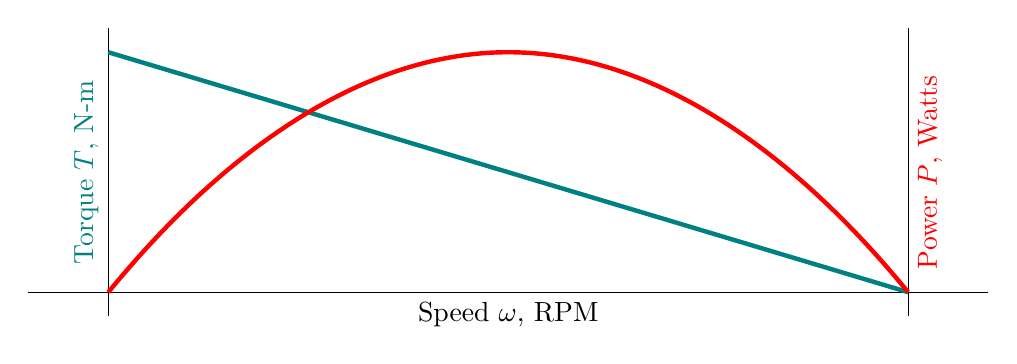
\begin{tikzpicture}[x=4.0in,y=1.2in]
  %\fill[lightgray] (1.0,0)--(0,1.0)--(0,0)--cycle;
  \draw[black] (-0.1,0)--(1.1,0) node[pos=0.5,below]{Speed $\omega$, RPM};
  \draw[black] (0,-0.1)--(0,1.1) node[pos=0.5,above,rotate=90,teal]{Torque $T$, N-m};
  \draw[black] (1,-0.1)--(1,1.1) node[pos=0.5,below,rotate=90,red]{Power $P$, Watts};

  \draw[teal, ultra thick] (1.0,0)--(0,1.0);
  \draw[red, ultra thick] (0,0) parabola bend (0.5,1.0) (1.0,0.0) ;
  
  % IMPROVEMENT: Peak power
\end{tikzpicture}
\caption{Power forms a parabolic curve with speed.}
\end{figure}

From this we can see that the peak power is produced at half of free speed. This is also half of torque.

Current ($I$) is how much electricity is drawn. It varies proportionally to torque, so

\begin{align} \label{eq:motor_current_curve}
  I = C T \nonumber \\
  I = C T_{stall} \frac{\omega_{free}-\omega}{\omega_{free}}
\end{align}

\begin{figure}[H] \centering
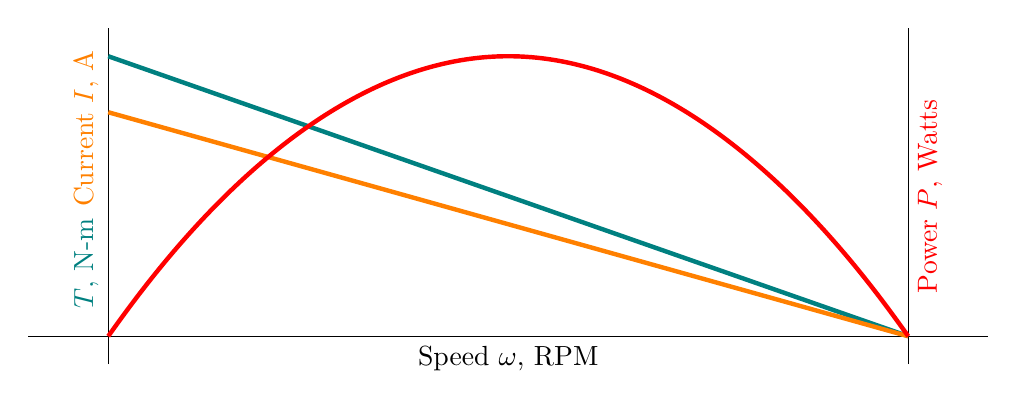
\begin{tikzpicture}[x=4.0in,y=1.4in]
  %\fill[lightgray] (1.0,0)--(0,1.0)--(0,0)--cycle;
  \draw[black] (-0.1,0)--(1.1,0) node[pos=0.5,below]{Speed $\omega$, RPM};
  \draw[black] (0,-0.1)--(0,1.1) node[pos=0.3,above,rotate=90,teal]{$T$, N-m} node[pos=0.7,above,rotate=90,orange]{Current $I$, A};
  \draw[black] (1,-0.1)--(1,1.1) node[pos=0.5,below,rotate=90,red]{Power $P$, Watts};

  \draw[teal, ultra thick] (1.0,0)--(0,1.0);
  \draw[orange, ultra thick] (1.0,0)--(0,0.8);
  \draw[red, ultra thick] (0,0) parabola bend (0.5,1.0) (1.0,0.0) ;
  
  % TODO: Label stall current
\end{tikzpicture}
\caption{Current varies with torque.}
\end{figure}

Efficiency ($\eta$) is a ratio of how much mechanical energy is produced per electrical energy spent.

\begin{equation} \label{eq:motor_efficiency_curve}
  \eta = \frac{P_{mech}}{P_{elec}} = \frac{T-M_{friction} \omega}{V I}
  = \frac{[T_{stall} \ \frac{(\omega_{free}-\omega)}{\omega_{free}} - M_f] \omega}{V\ C\ T_{stall} \frac{(\omega_{free}-\omega)}{\omega_{free}}} \nonumber
\end{equation}

Indeed an ugly equation, let's just plot it with some semi-realistic values.

\begin{figure}[H] \centering
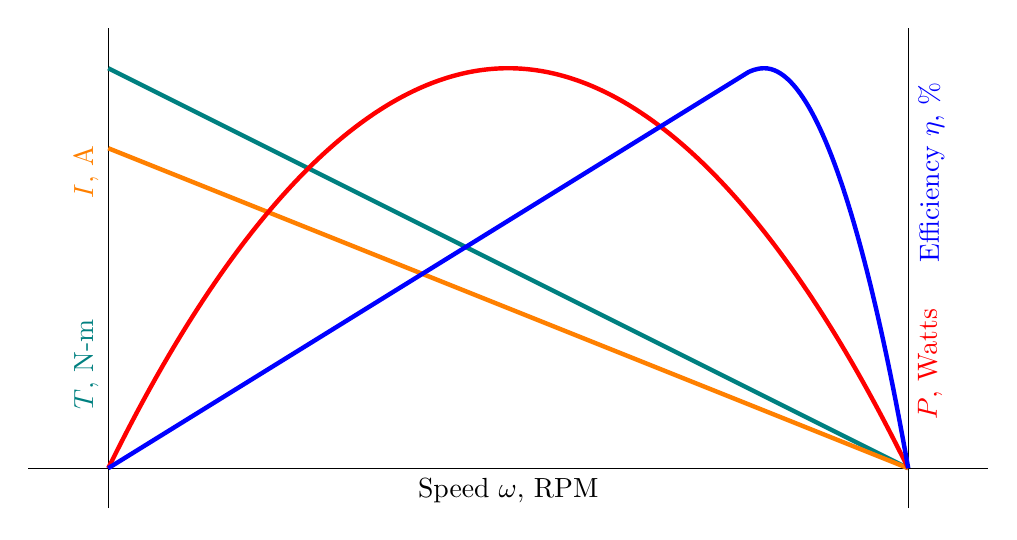
\begin{tikzpicture}[x=4.0in,y=2.0in]
  %\fill[lightgray] (1.0,0)--(0,1.0)--(0,0)--cycle;
  \draw[black] (-0.1,0)--(1.1,0) node[pos=0.5,below]{Speed $\omega$, RPM};
  \draw[black] (0,-0.1)--(0,1.1) node[pos=0.3,above,rotate=90,teal]{$T$, N-m}
  node[pos=0.7,above,rotate=90,orange]{$I$, A};
  \draw[black] (1,-0.1)--(1,1.1) node[pos=0.3,below,rotate=90,red]{$P$, Watts}
  node[pos=0.7,below,rotate=90,blue]{Efficiency $\eta$, \%};

  \draw[teal, ultra thick] (1.0,0)--(0,1.0);
  \draw[orange, ultra thick] (1.0,0)--(0,0.8);
  \draw[red, ultra thick] (0,0) parabola bend (0.5,1.0) (1.0,0.0) ;
  \draw[blue, ultra thick] (0,0)--(0.8,0.99) parabola bend (0.82,1.0) (1.0,0.0) ;
\end{tikzpicture}
\caption{Complete motor curve.}
\end{figure}

In summary:
\begin{asparaitem}
	\item Motors produce less and less torque as they spin up.
	\item No power is produced when the motor is at maximum speed or maximum torque.
	\item Maximum power is produced at 50\% of maximum speed, which is also at 50\% of maximum torque.
	\item Maximum efficiency occurs somewhere between 75\% and 90\% of free speed.
\end{asparaitem}


\section{Comparing Motor Types}

\begin{table}[H]
\begin{tabular}{lll}
                      & \textit{Brushed DC}   & \textit{Brushless DC}                \\
\textbf{Efficiency}            & Low          & High                        \\
\textbf{Mechanical Robustness} & Medium       & High                        \\
\textbf{Electronic Complexity} & Low          & High                        \\
\textbf{Position Control}      & Not inherent & \begin{tabular}[c]{@{}l@{}}May have\\ integrated encoder\end{tabular} \\
\textbf{Cost}                  & Low          & Medium                     
\end{tabular}
\caption{Motor types at a glance}
\end{table}


\chapter{Design Principles}
\section{Structural}
\subsection{Load paths (axial not bending)}
\subsection{Big sections for bending/torque}
\subsection{Spread the base}
\section{Error}
\subsection{Abbe (sine) error}
\subsection{Tolerance stacking (minimize number of components)}
\section{Time-Related Failures}
\subsection{Loosening (see locking mechanisms)}
\subsection{Fatigue}


\chapter{Applied Systems}

 {\slshape \scshape ``Complex is better than complicated." - The Zen of Python}
 \\

\section{Intakes}
\subsection{Beater bars}
\subsection{Side wheels}
\subsection{Vectored Intake Wheels}

\section{Indexers}
\subsection{Conveyors}
\subsection{Hoppers}
\subsection{Rotary hoppers}

\section{Lifts}
\subsection{Elevators - Cascade and Continuous}
\subsection{Obscure 4 bar}
\subsection{Parallel 4 bar}
\subsection{Virtual 4 bars}
\subsection{6 8 etc. bars}
\subsection{Double reverse 4 bar}

\section{Latches}
\subsection{Latches}
\subsection{Overcenter mechanisms}

\section{Shooters}
\subsection{Flywheel-based launcher}
\subsection{Catapults and Punches}
\subsection{Winch and Release vs. Choo-Choo vs. Cam}

\section{Drivetrains}
\subsection{Tanks}
\subsection{Omnis}
\subsection{Transformers}
\subsection{Swerve Modules}



\chapter{Choosing Gear Ratios}

 {\slshape \scshape ``Power is worthless, if improperly wielded"}
 \\

If we have a motor with a pinion of $N_m$ teeth, mating with a driven gear of $N_d$ teeth, we would achieve a gear ratio of

\begin{align}
  G = \frac{N_d}{N_m} = \frac{\omega_m}{\omega_d} = \frac{T_d}{T_m}
\end{align}

This also works with belts or sprockets and chain (though you may need to keep an eye on the direction of rotation, as gears can reverse the direction of rotation).


\begin{figure}[H] \centering
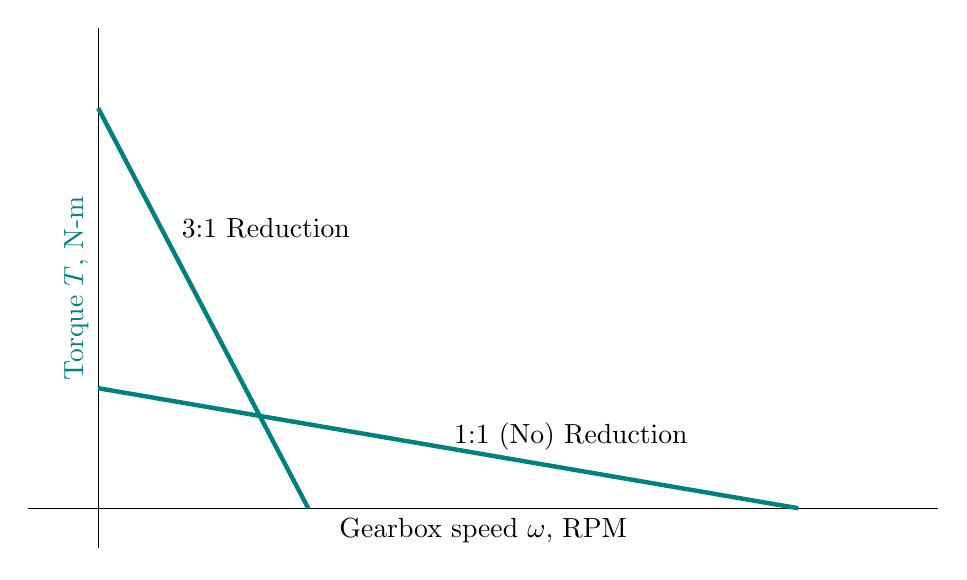
\begin{tikzpicture}[x=3.5in,y=2.0in]
  %\fill[lightgray] (1.0,0)--(0,1.0)--(0,0)--cycle;
  \draw[black] (-0.1,0)--(1.2,0) node[pos=0.5,below]{Gearbox speed $\omega$, RPM};
  \draw[black] (0,-0.1)--(0,1.2) node[pos=0.5,above,rotate=90,teal]{Torque $T$, N-m};

  \draw[teal, ultra thick] (1.0,0)--(0,0.3) node[pos=0.6, right, black]{\ \ \ \ \ \ \ 1:1 (No) Reduction};
  \draw[teal, ultra thick] (0.3,0)--(0,1.0) node[pos=0.7, right, black]{\ 3:1 Reduction};
\end{tikzpicture}
\caption{A 3:1 gear reduction shifts the effective motor curve of a gearbox.}
\end{figure}

The 3:1 ratio reduces maximum speed, but increases the maximum torque. It also changes the RPM at which maximum power and efficiency occur. A gearbox that has too much gear-down:
\begin{asparaitem}
	\item Quickly gets up to its maximum speed and remains there throughout the majority of its action.
	\item Operates beyond the speed necessary for peak efficiency of the motor.
	\item Operates for too long, wasting electrical power.
\end{asparaitem}

Whereas a gearbox that is not geared down enough:
\begin{asparaitem}
	\item Operates below the speed necessary for peak power or efficiency of the motor.
	\item Pulls excessive current, wasting electrical power.
	\item May not even move at all in the first place, lacking the strength to overcome load placed on it.
\end{asparaitem}

But how do we know that we've geared appropriately? We could definitely test all the different ratios, gather all the operating data, and then draw a conclusion... or we could do some pre-emptive math. Don't worry- you don't even need to get your hands too dirty. All of the rough stuff has been done already- you just need to know how to use the design applications to get the answer you want.

But knowing roughly what's going on is important. There's an old joke in engineering,

 {\slshape \scshape ``All data is wrong. But this data, having gone through an incredibly sophisticated computer, is somehow ennobled and none dare question it."}
 
 Which roughly translates to: ``You can't just mash buttons and trust the results".

\section{Developing a Generalized Mechanism Model}

\subsection{The Simple Flywheel Case}

Let's examine a simple case of a motor accelerating a flywheel. This is also (essentially) the same as any system with no friction or gravity-fighting (like an ideal drivetrain).
	
	\begin{figure}[H] \centering
	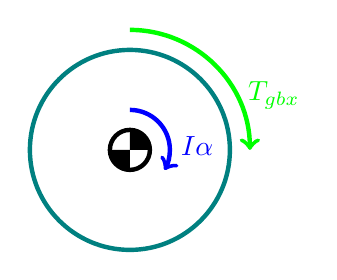
\begin{tikzpicture}[x=1.0in,y=1.0in]
		\draw[ultra thick] (0,0) circle (0.1);
		\fill[black] (0,0.1)--(0,0)--(0.1,0) arc[start angle=0, end angle=90, radius=0.1]--cycle;
		\fill[black] (0,-0.1)--(0,0)--(-0.1,0) arc[start angle=180, end angle=270, radius=0.1]--cycle;
		\draw[ultra thick, teal] (0,0) circle (0.5);
		
		%\draw[ultra thick, red, ->] (0,0.6) arc[start angle=90, end angle=180, radius=0.6] node[pos=0.7,left]{$M_{resist}$};
		\draw[ultra thick, green, ->] (0,0.6) arc[start angle=90, end angle=0, radius=0.6] node[pos=0.7,right]{$T_{gbx}$};
		
		\draw[ultra thick, blue, ->] (0,0.2) arc[start angle=90, end angle=-30, radius=0.2] node[pos=0.7,right]{$I \alpha$};
	\end{tikzpicture}	
	\caption{Free-body diagram of the flywheel}
	\end{figure}	
	
	We can apply conservation of angular momentum to the flywheel.
	\begin{align}
		\sum M &= I \alpha + \cancelto{0 \ \mbox{(no mass transfer)}}{\sum \dot{m}(...)} \\
		T_{gbx} &= I \ \alpha_{wheel}
	\end{align}
	
	This tells us about the rate of acceleration $\alpha$, but what about the velocity $\omega$? 
		
	\begin{align}
		\alpha_{wheel} &= \frac{d \omega_{wheel}}{dt} \\
		\omega_{motor} &= G \omega_{wheel} \\
		G T_{stall} \frac{\omega_{free} - \omega}{\omega_{free}} &= \frac{I}{G} \frac{d \omega}{dt}
	\end{align}
	
		This is a "differential equation" ($\frac{d \omega}{dt}$ and $\omega$ appear in the same equation). These are tricky to solve. \textit{There be dragons ahead. If you don't care to know all the intricate mathy details, skim ahead. I don't blame you.}
		
	\subsection{The Full-Blown Calculus Approach}
	
	We can solve differential equations with calculus!	
	\begin{align}
		\mbox{let }& &B  &= \frac{G^2 T_{stall}}{I} \\
		\mbox{Substitute: }& & B\ \frac{\omega_{free} - \omega}{\omega_{free}} &= \frac{d \omega}{d t} \\
		\mbox{Separate and integrate: }& & \int B\ dt &= \int \frac{\omega_{free}}{\omega_{free} - \omega} d \omega \\
		\mbox{Compute integral (introduces $C$): }& & B t + C &= -\omega_{free}\ ln[\omega_{free} - \omega] \\
		\mbox{Solve for $\omega$: }& & \omega &= \omega_{free} - C\ e^{-\frac{B t}{\omega{max}}} \\
		\mbox{Solve for C with initial condition }& & \omega(0) &= 0 \rightarrow C = \omega_{free} \\
		& &\omega &= \omega_{free}\ [1 - e^{-\frac{G^2\ T_{stall}\ t}{I\ \omega{max}}}] \\
		& &\omega_{gbx} &= \frac{\omega_{free}}{G}\ [1 - e^{-\frac{G^2\ T_{stall}\ t}{I\ \omega{max}}}]
	\end{align}	
	
	If we plot this algebraic solution with some generalized values, we can start to investigate what it really means.	
	
	\begin{figure}[H] \centering
	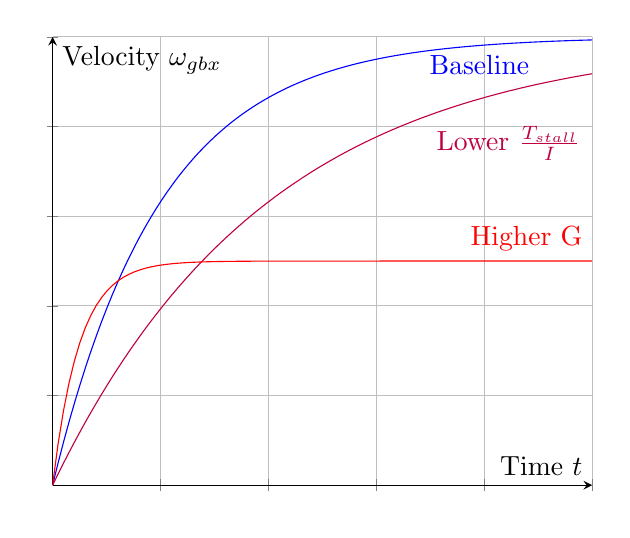
\begin{tikzpicture}[x=3.0in,y=1.5in]
		%\draw[gray] (0,0)--(3,0) node[pos=0.5,below,black]{Time $t$};
		%\draw[gray] (0,0)--(0,2) node[pos=0.5,above,rotate=90,black]{Ang. Velocity $\omega_{gbx}$};
		
		%\draw[red] (0,0)
		
		\begin{axis}[grid=both,
          xmax=5,ymax=1,
          xticklabel=\empty, yticklabel=\empty,
          axis lines=middle,
          restrict y to domain=-7:12,
          xlabel={Time $t$},
          ylabel={Velocity $\omega_{gbx}$}
          ]
		\addplot[blue,domain=0:5,samples=100]  {1*(1-exp(-1^2*x))} node[pos=0.8,below] {Baseline};
		\addplot[purple,domain=0:5,samples=100]  {1*(1-exp(-1^2/2*x))} node[pos=0.7,below right] {Lower $\frac{T_{stall}}{I}$};
		\addplot[red,domain=0:5,samples=100]  {1/2*(1-exp(-2^2*x))} node[above left] {Higher G};
		\end{axis}
	\end{tikzpicture}
	\caption{Flywheel example solution, with different representative parameters}
	\end{figure}
		
	This assumes that there is no constant load, or friction.
	This behavior is generally true, but not exactly true.
	
	\subsection{A Brute-Force Approach}
	We don't need to solve that differential equation using calculus. Or math. We can use basic arithmetic and computers to simulate it! We can do this with a 'numeric differential equation solver', like Euler's Method:
	\begin{equation}
		\frac{d}{dt} f(t) \approx \frac{\Delta f(t)}{\Delta t}
	\end{equation}\begin{equation}
		f(t_{i+1}) = f(t_{i}) + \frac{d}{dt}[f(t_{i})]\ {\Delta t}
	\end{equation}
	
	\begin{figure}[H]
		\includegraphics[width=0.35\textwidth]{imgs/euler_method.png}
		\caption{Graphical representation of Euler's method.}
	\end{figure}
	
	Another way of putting it... "the next value is the current value, plus the rate of change times the timestep of the simulation". 	We just need to get an expression for the $\frac{d}{dt}f(t)$ we are interested in, and write some code that will repeat this process with a small enough $\Delta t$. This process is sometimes called 'discretization' since we are taking a continuous field of time $t$ and separating it into little $\Delta t$ chunks.	
		
	Let's go back to our flywheel example, and add resistance $M_{resist}$ to it. This $M_{resist}$ can be anything- it can represent friction, air resistance, a spring, you name it! The numeric simulation approach makes this trivial.
	
	\begin{figure}[H] \centering
	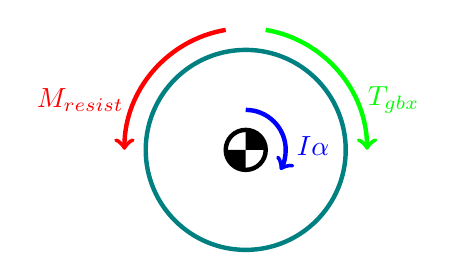
\begin{tikzpicture}[x=1.0in,y=1.0in]
		\draw[ultra thick] (0,0) circle (0.1);
		\fill[black] (0,0.1)--(0,0)--(0.1,0) arc[start angle=0, end angle=90, radius=0.1]--cycle;
		\fill[black] (0,-0.1)--(0,0)--(-0.1,0) arc[start angle=180, end angle=270, radius=0.1]--cycle;
		\draw[ultra thick, teal] (0,0) circle (0.5);
		
		\draw[ultra thick, red, ->] (-0.1,0.6) arc[start angle=99.6, end angle=180, radius=0.608] node[pos=0.7,left]{$M_{resist}$};
		\draw[ultra thick, green, ->] (0.1,0.6) arc[start angle=80.4, end angle=0, radius=0.608] node[pos=0.7,right]{$T_{gbx}$};
		
		\draw[ultra thick, blue, ->] (0,0.2) arc[start angle=90, end angle=-30, radius=0.2] node[pos=0.7,right]{$I \alpha$};
	\end{tikzpicture}	
	\caption{Free-body diagram for the flywheel, with additional resistance $M_{resist}$.}
	\end{figure}
	
	We can go through and repeat the same analysis as before.
	\begin{align}
		\sum M &= I \alpha + \cancelto{0 \ \mbox{(no mass transfer)}}{\sum \dot{m}(...)}  \\
		T_{gbx} - M_{resist} &= I \alpha_{wheel} \\
		\alpha_{wheel} &= \frac{d}{dt} \omega_{wheel} \\
	\end{align}
	
We can solve to yield the equations we need to perform Newton's Method:	
	
	\begin{align}
		\frac{d}{dt} \omega_{wheel} &= \frac{T_{gbx} - M_{resist}}{I} \\
		\frac{d}{dt} \theta_{wheel} &= \omega_{wheel}
	\end{align}
	
	My \href{http://thaddeus-maximus.github.io/swissarmyengineer/}{\color{red}\underline{Swiss Army Engineer}} tool contains a Simple Mechanism Calculator you can use to leverage these physics.

	
\section{Using the Simulations: Analysis/Optimization Examples}

Let's consider an example drivetrain, with 4 NEOs, 8" diameter wheels, weighing about 143 pounds, meeting 30 N of resistive force. We want to go 10 meters. We have two gear ratio options to consider: a 10:1 gearbox, and a 7:1 gearbox. Which should we pick?

Before you look at the plots, go to the simulator and plug in those values, see if you can come up with an answer of which gets to the destination faster.

\clearpage
	
	\begin{figure}[H] \centering
	\includegraphics[width=0.8\textwidth]{imgs/thsae_1.png}
	\caption{Baseline simulation, G = 10, t = 2.03 s}
	\end{figure}
	
	\begin{figure}[H] \centering
	\includegraphics[width=0.8\textwidth]{imgs/thsae_2.png}
	\caption{Alternative simulation, G = 7, t = 1.88 s}
	\end{figure}
	
	It looks like the ratio of 7 will get to our destination faster!
	
	However, maybe this isn't our only concern. Drivetrains are complex mechanisms with many objectives (as we'll discuss later). The G = 10 case has lower current consumption (almost half!) in this maneuver. It has more initial pushing power. It also gets to positions less than 3 meters away faster. There are a lot of tradeoffs!
	
\chapter{Going Forth}

 {\slshape \scshape ``Learn the rules like a pro, so you can break them like an artist." - Pablo Picasso}
 \\


\end{document}
